\documentclass{article}

\usepackage{pdfpages}

\usepackage{caption}
\usepackage{subcaption}

\usepackage{float}
\usepackage{geometry}
\geometry{
	a4paper,
	total={170mm,257mm},
	left=20mm,
	right=20mm,
	top=10mm,
}

\usepackage{physics, amsmath, amsfonts, fixmath, tikz, pgf, multirow, hyperref, amsfonts,amssymb, mathtools, physics, xcolor, siunitx}

\title{Chaos in Hodgkin Huxley model\\ Computational Neuroscience}
\author{Arshia Razavi\\30190016}

\begin{document}
	\maketitle
	
	\section{Introduction}
		In this report I am exploring Hodgkin Huxley model in order to find chaotic behaviors when control parameter is external current I and is constant respect to time.
		The Hodgkin Huxley model for a single neuron with original parameters [3]: 
		\begin{align*}
			\dot{v} &= I - (120m^3h(v+115) + 36n^4(v-12) + 0.3(v+10.599))\\
			\dot{m} &= (1-m) \Psi(\frac{v+25}{10}) - m(4exp\frac{v}{18})\\
			\dot{n} &= (1-n)0.1\Psi(\frac{v+10}{10})-n(0.125exp\frac{v}{80})\\
			\dot{h} &= (1-h)0.07exp(\frac{v}{20}) -\frac{h}{1+exp\frac{v+30}{10}}
		\end{align*}
		Where v is the membrane potential and (m,n,h) are representatives of ions' channels activity. This system has a bifurcation diagram over control parameter of I which is shown in figure 1 [1]. Spiking regime exists for $I > I_{th} \approx 6.26$ which $I=I_{th}$ is a saddle node bifurcation where two stable and unstable limit cycles arises at that point. Stability of fixed point is guaranteed for $I < I_{Hopf}$ where at $I = I_{Hopf} \approx 9.8$ stable fixed point merges with an unstable limit cycle and forms a new unstable fixed point. The system also has a period doubling bifurcation at $I_{PD}$ which is near s area (red curve) in the figure 1. \\
		As mentioned in paper [1] we expect chaos in s area. By using Poincare map (Discrete map) and finding Smale horseshoe, existence of chaos is proved. 
		
		% TODO: \usepackage{graphicx} required
		\begin{figure}[H]
			\centering
			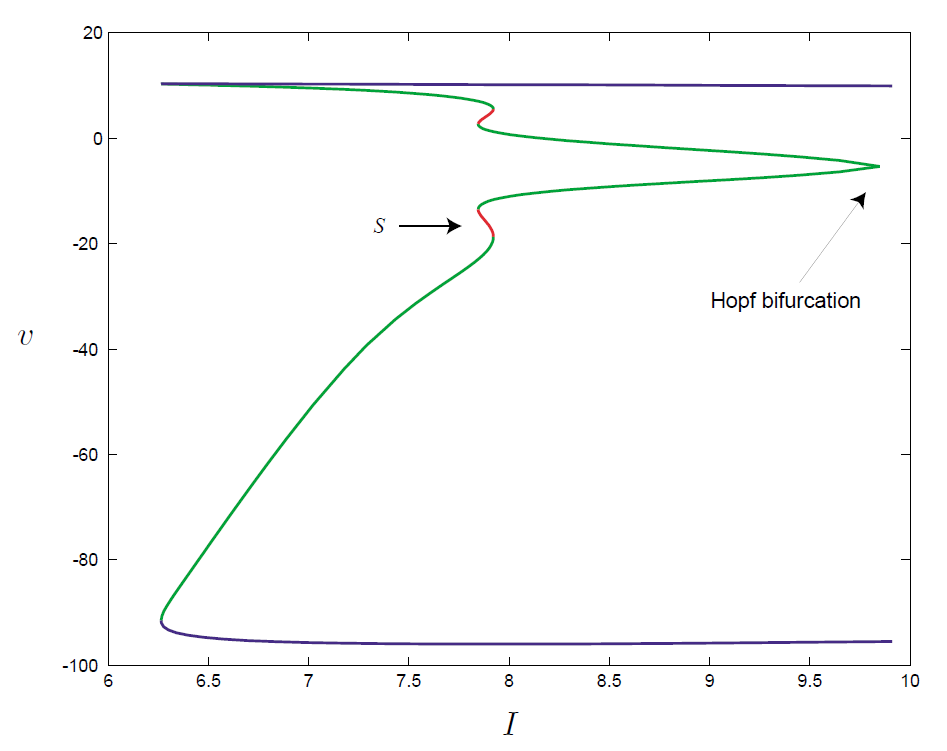
\includegraphics[width=0.5\linewidth]{Bifurcation_Diagram}
			\caption{The amplitude of periodic orbits in the Hodgkin–Huxley model as a function of input
				current. Maximum and minimum values of v are plotted for each periodic orbit. Stable periodic orbits are
				shown in blue; those shown in green have a single positive unstable eigenvalue, while those shown in red have
				either two unstable eigenvalues or a negative unstable eigenvalue. [1]}
			\label{fig:bifurcationdiagram}
		\end{figure}
		
	\section{Saddle node bifurcation and amplitudes of stable periodic orbit}
		In this part we are exploring saddle point bifurcation ($I_{SN}$ or $I_{th}$) :\\
		
		% TODO: \usepackage{graphicx} required
		\begin{figure}[H]
			\centering
			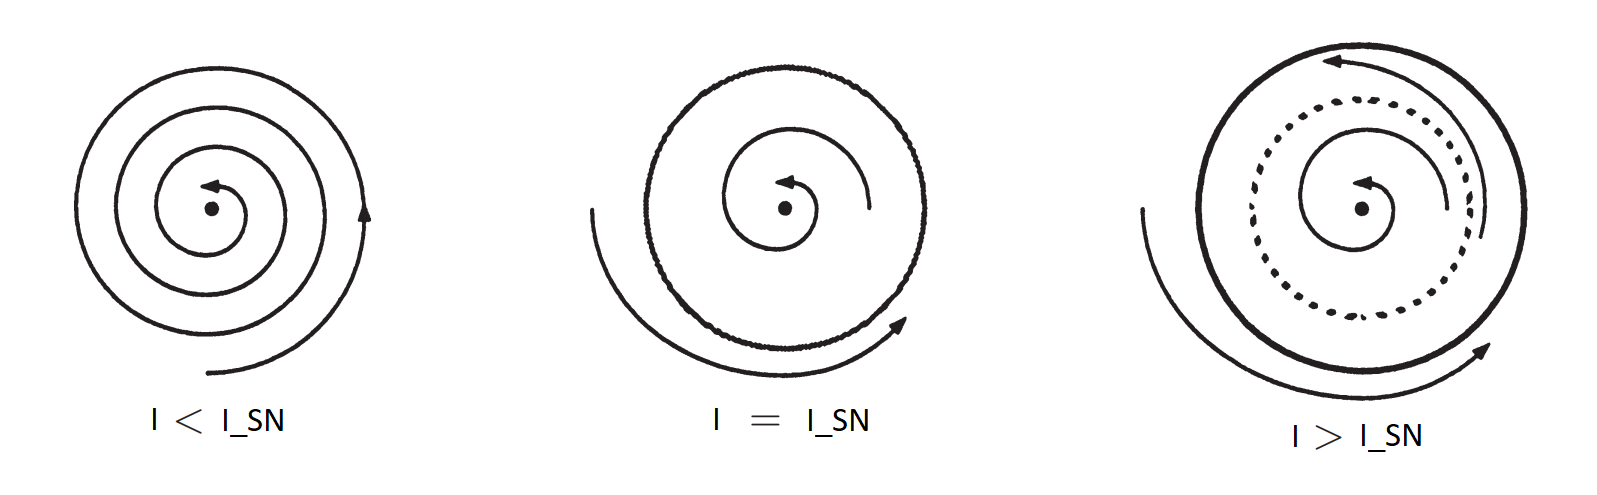
\includegraphics[width=0.7\linewidth]{saddle_node_bifurcation}
			\caption{Saddle Node Bifurcation Visualization [4]. Emergence of two unstable and stable limit cycles near together around an stable fixed point!}
			\label{fig:saddlenodebifurcation}
		\end{figure}
	
		\begin{figure}[H]
			\centering
			\begin{subfigure}{0.475\textwidth}
				\centering
				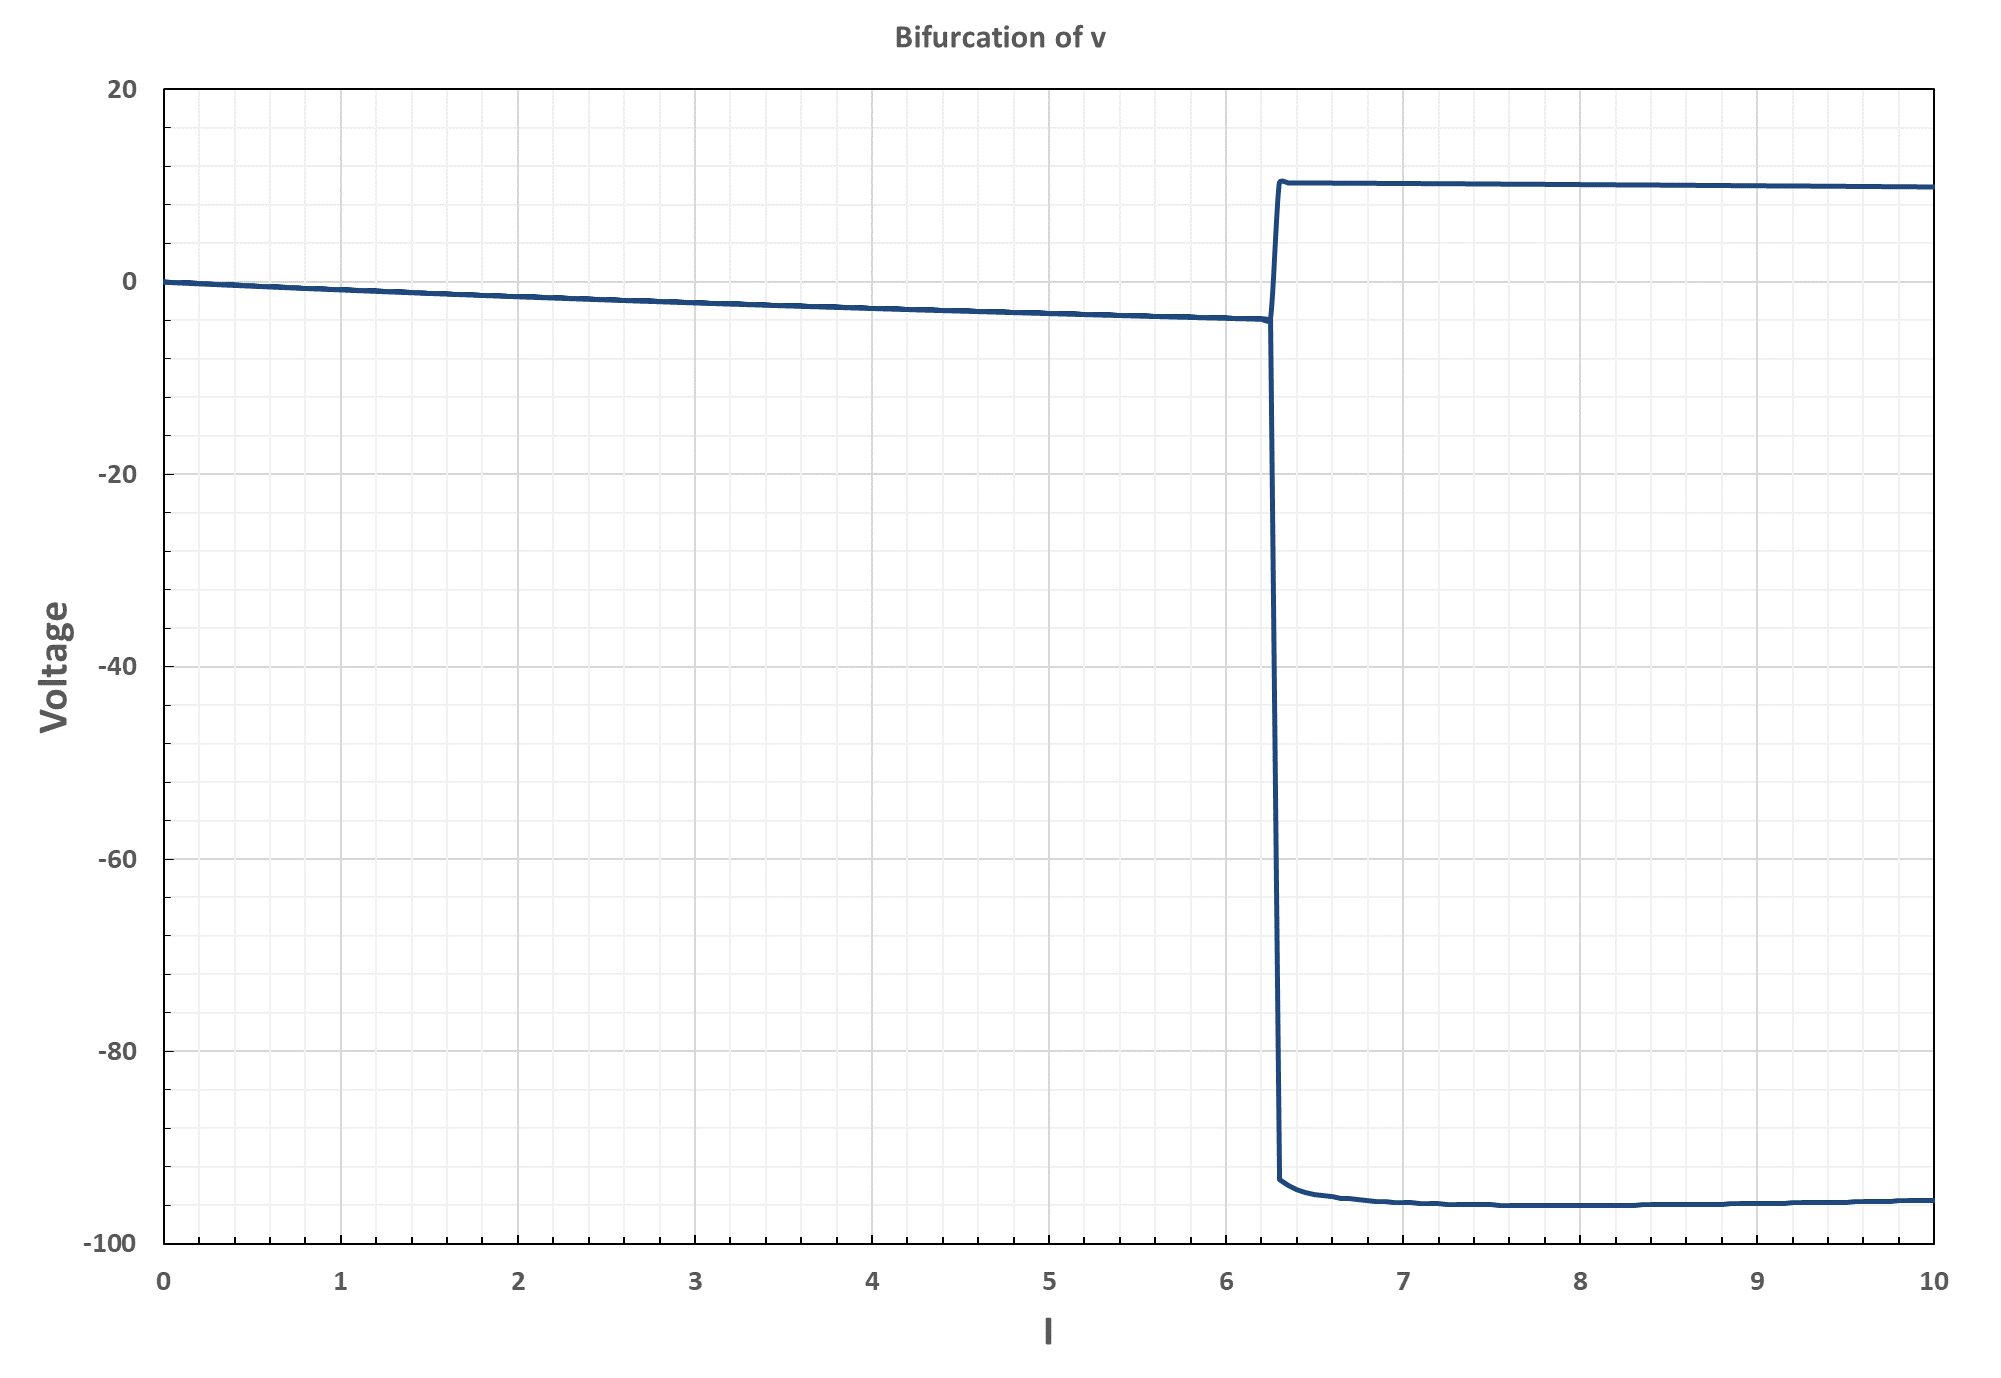
\includegraphics[width=\textwidth]{voltage}
				\caption{V - I}  
				\label{fig:mean and std of net14}
			\end{subfigure}
			\hfill
			\begin{subfigure}{0.475\textwidth}  
				\centering 
				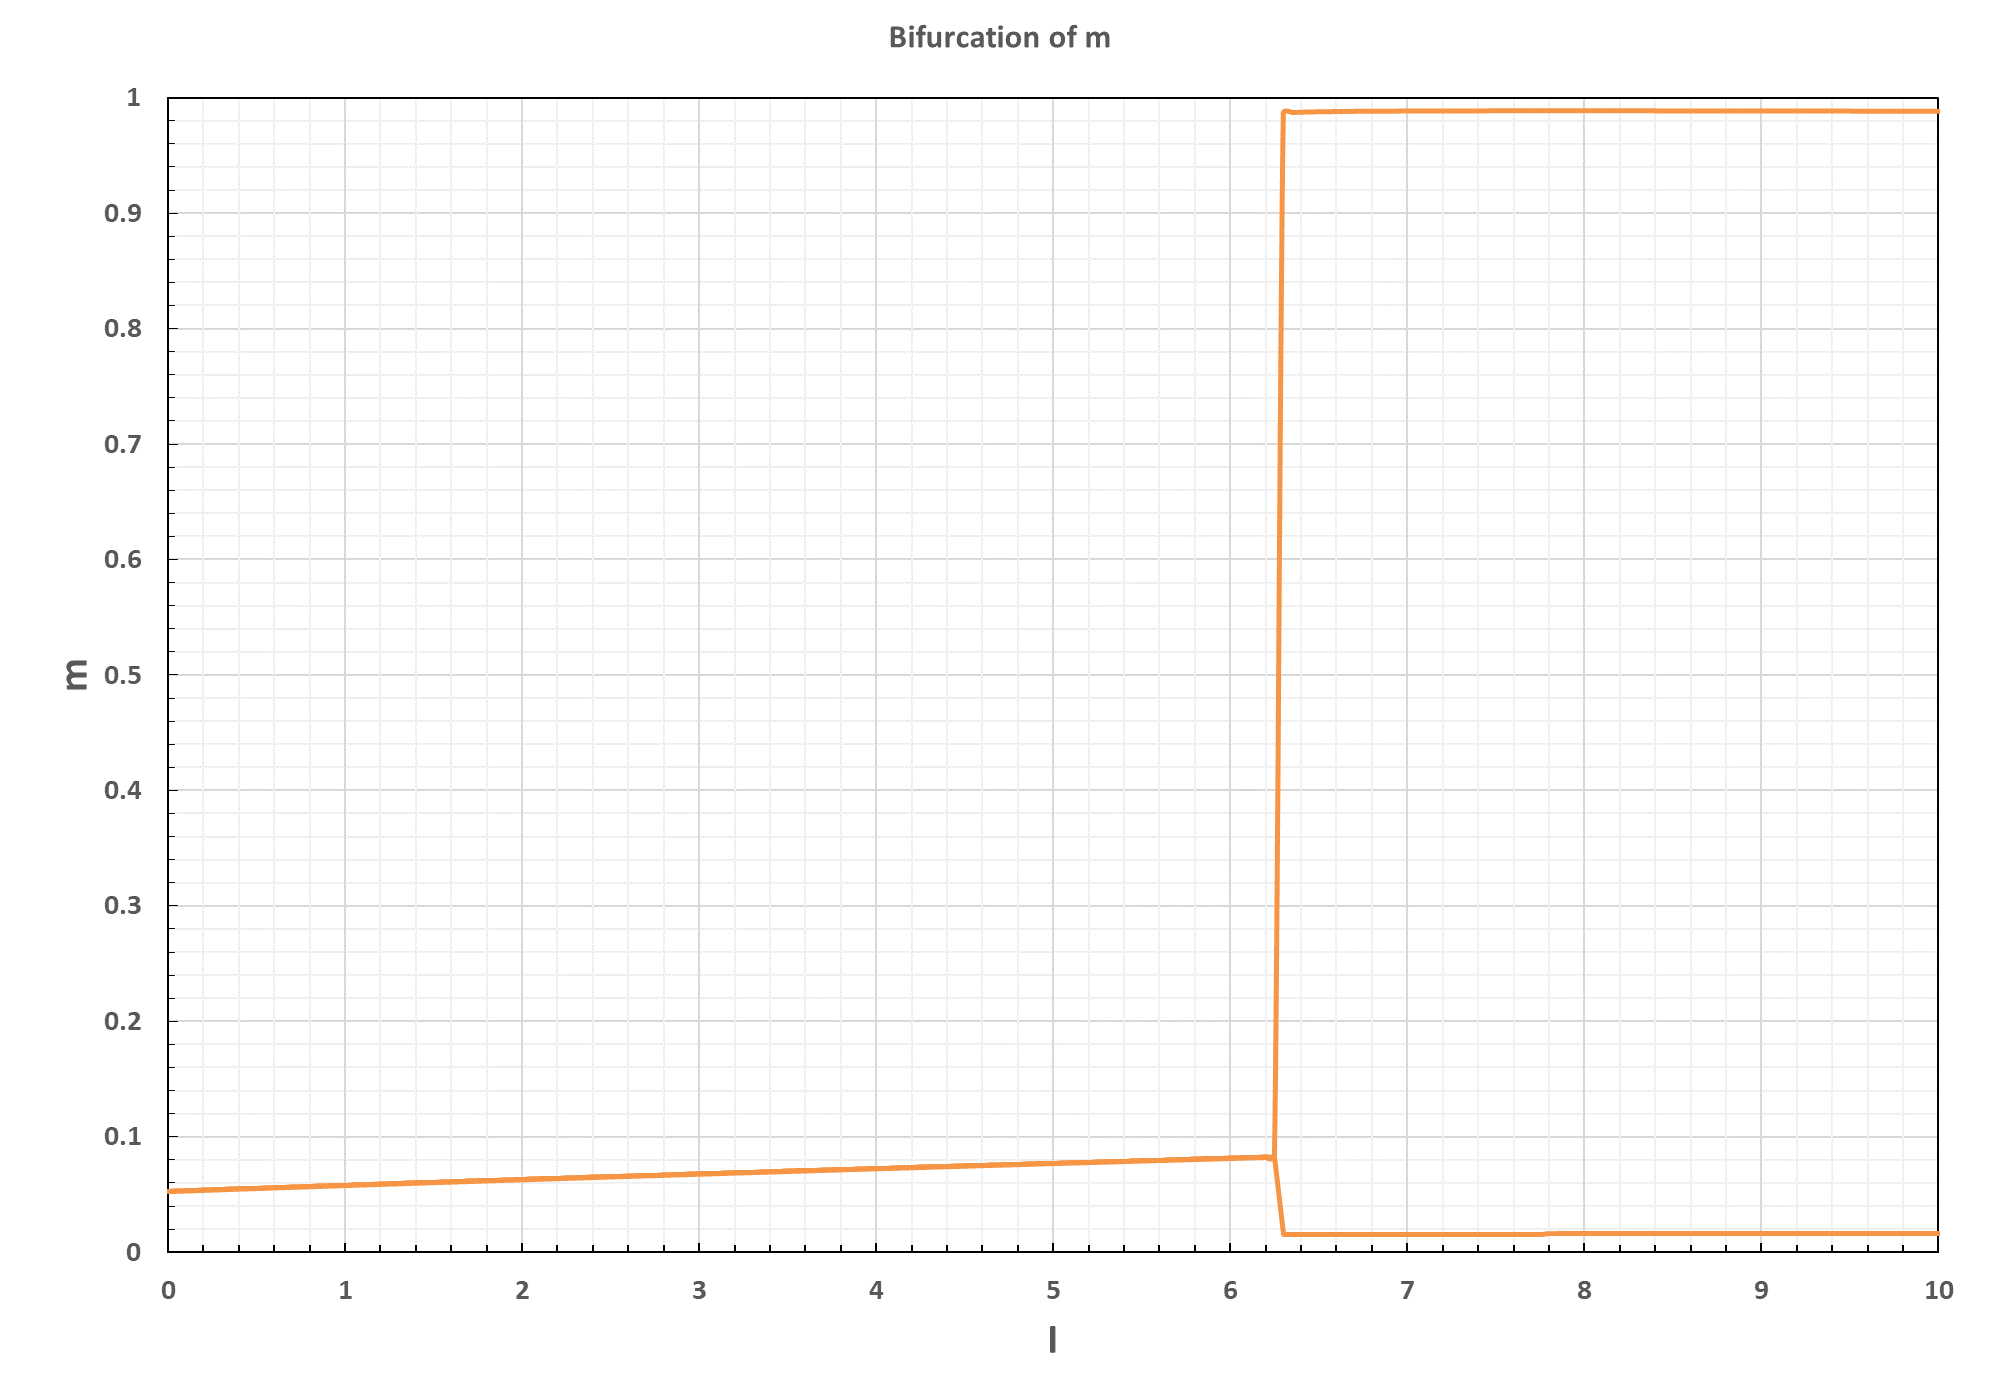
\includegraphics[width=\textwidth]{m}
				\caption{m - I}   
				\label{fig:mean and std of net24}
			\end{subfigure}
			\vskip\baselineskip
			\begin{subfigure}{0.475\textwidth}   
				\centering 
				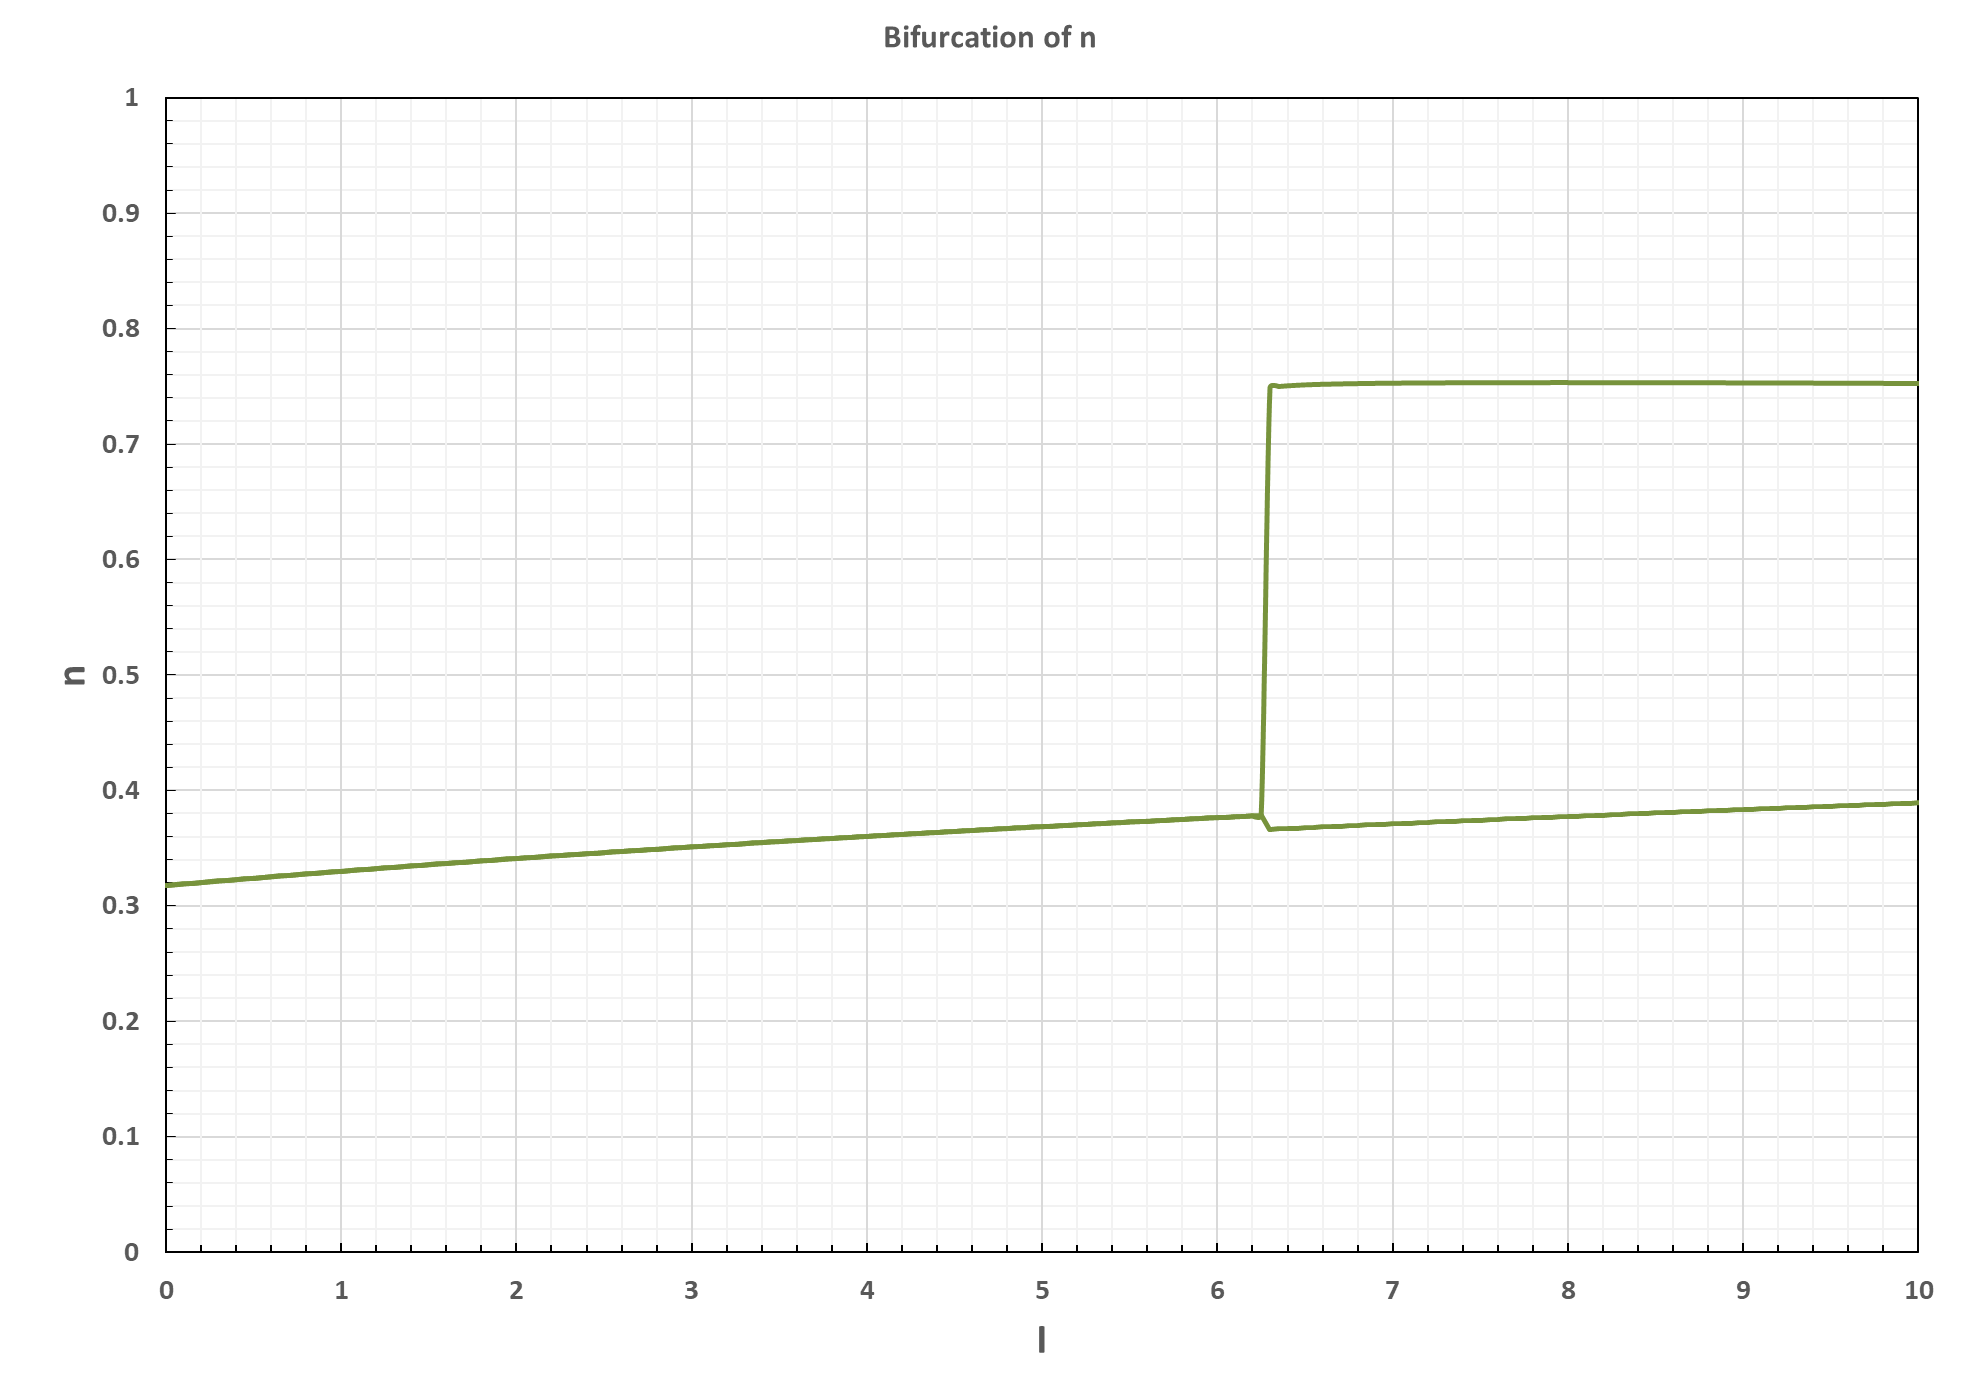
\includegraphics[width=\textwidth]{n}
				\caption{n - I}
				\label{fig:mean and std of net34}
			\end{subfigure}
			\hfill
			\begin{subfigure}{0.475\textwidth}   
				\centering 
				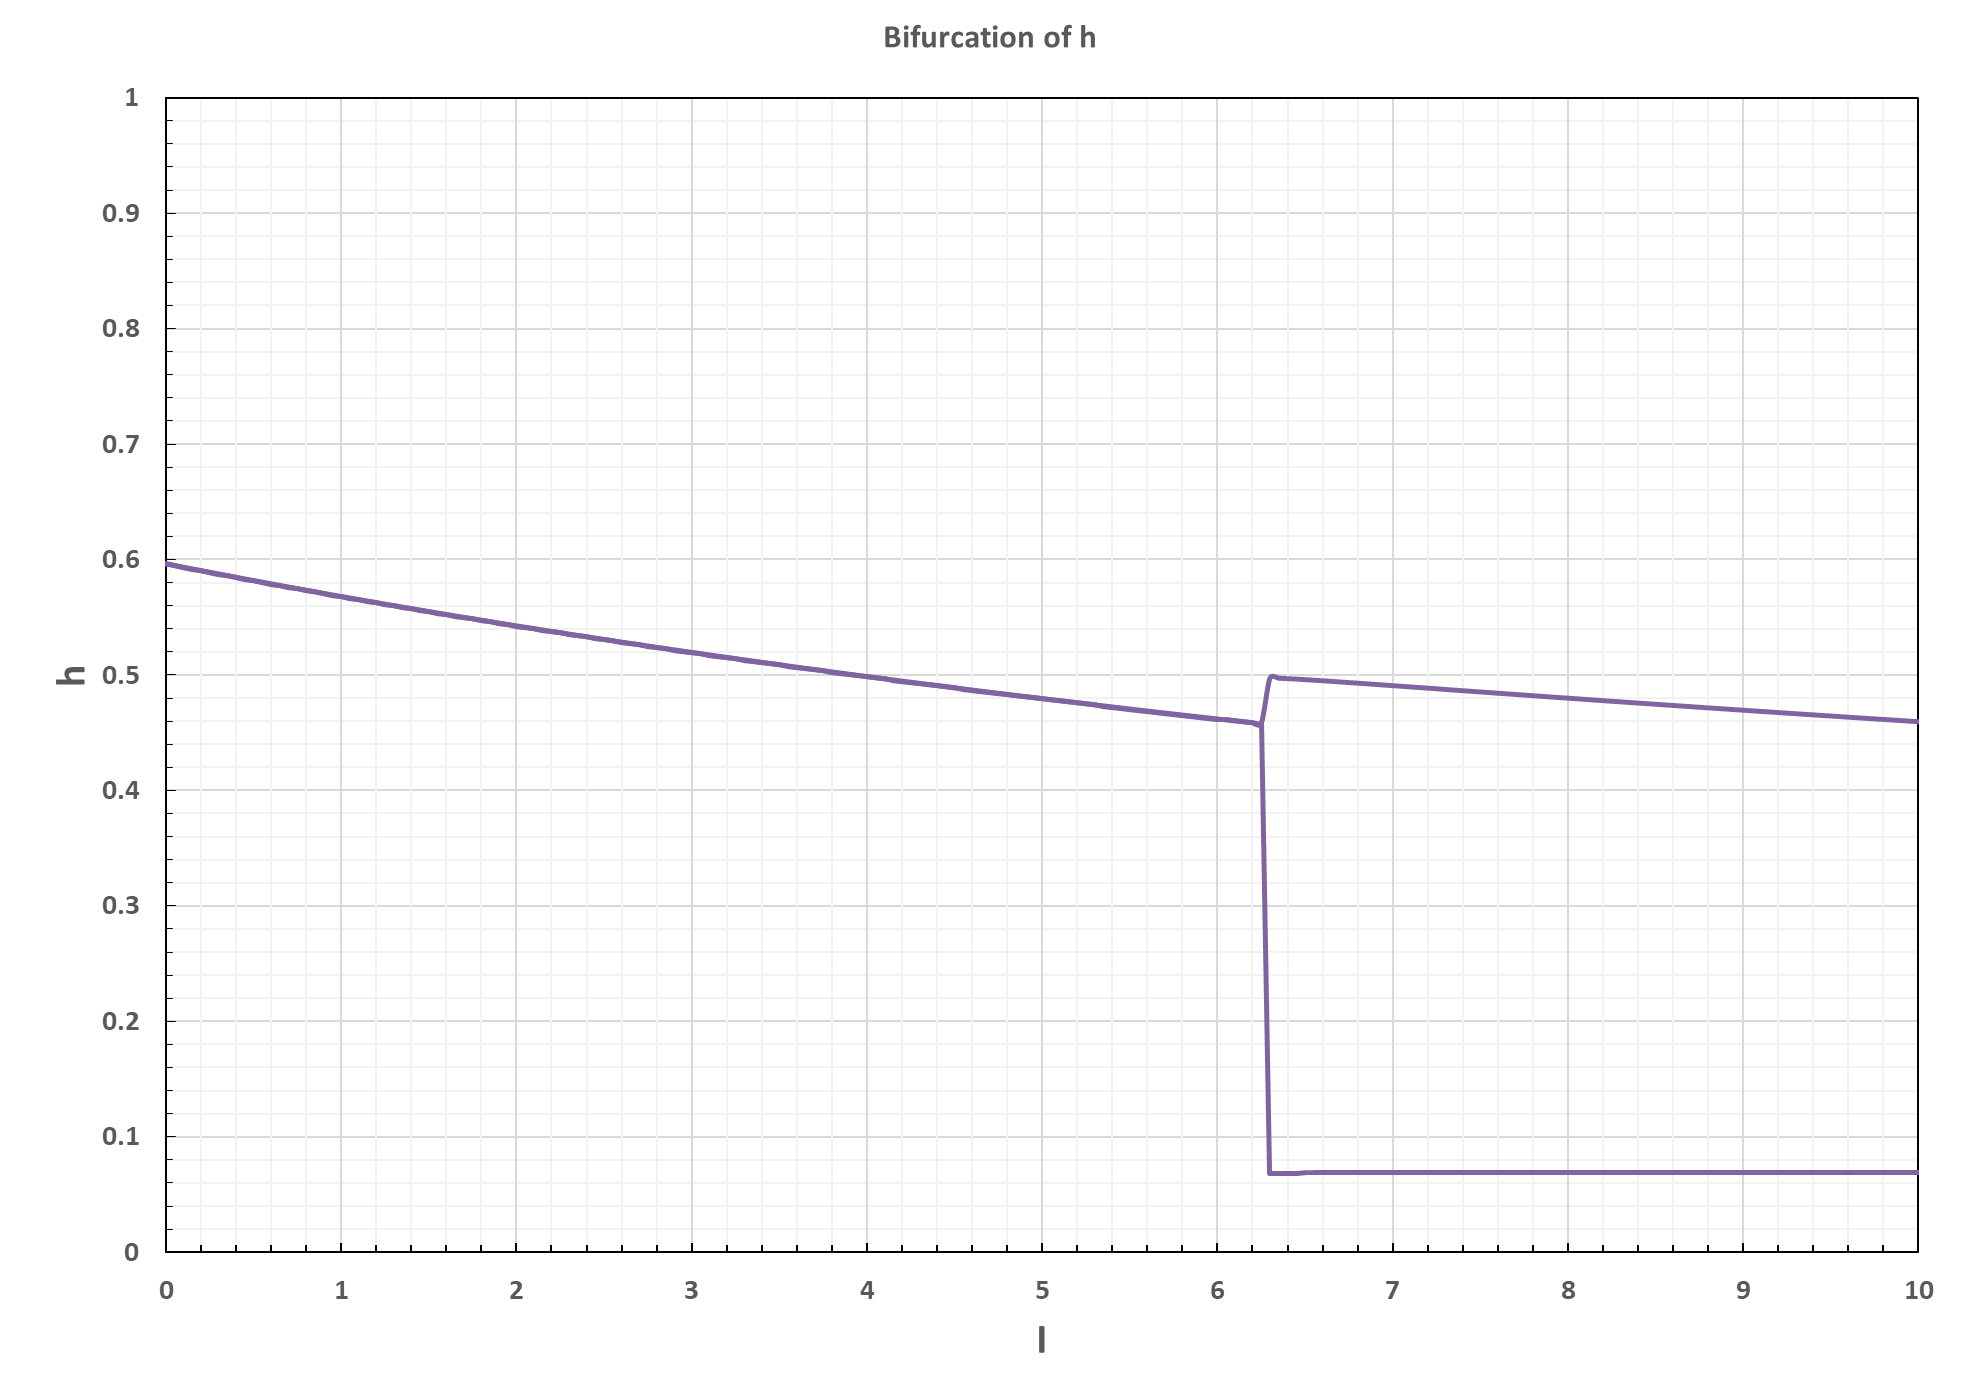
\includegraphics[width=\textwidth]{h}
				\caption{h - I}  
				\label{fig:mean and std of net44}
			\end{subfigure}
			\caption{Diagrams of maximum and minimum values of a stable motion for (v,m,n,h) in different currents. Stable limit cycle appears after the threshold current $I_{SN}=I_{th} \approx 6.26$. Unstable limit cycles are hard to detect and are not shown here. } 
			\label{fig:mean and std of nets}
		\end{figure}
	
		
		% TODO: \usepackage{graphicx} required
		\begin{figure}[H]
			\centering
			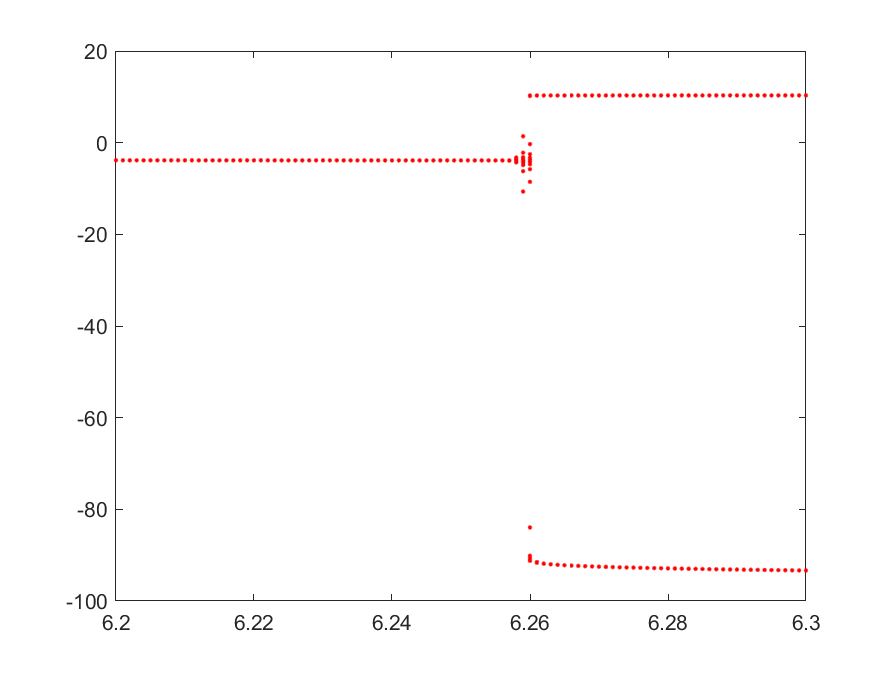
\includegraphics[width=0.7\linewidth]{fine_transition_current}
			\caption{Voltage versus I. Zoomed in diagram obtained form figure 3.a with high density simulation interval ($\Delta I$ = 0.001) to find $I_{SN} \approx 6.26$}
			\label{fig:finetransitioncurrent}
		\end{figure}
	
	\section{Sub-critical Hopf Bifurcation}
		In this part Sub-critical Hopf bifurcation has been computationally explored. The problem with unstable limit cycles is they are hard to detect and find, Because all trajectories diverge from them. As a result, $I_{SH}$ is not as precise as $I_{SN}$.
	
		% TODO: \usepackage{graphicx} required
		\begin{figure}[H]
			\centering
			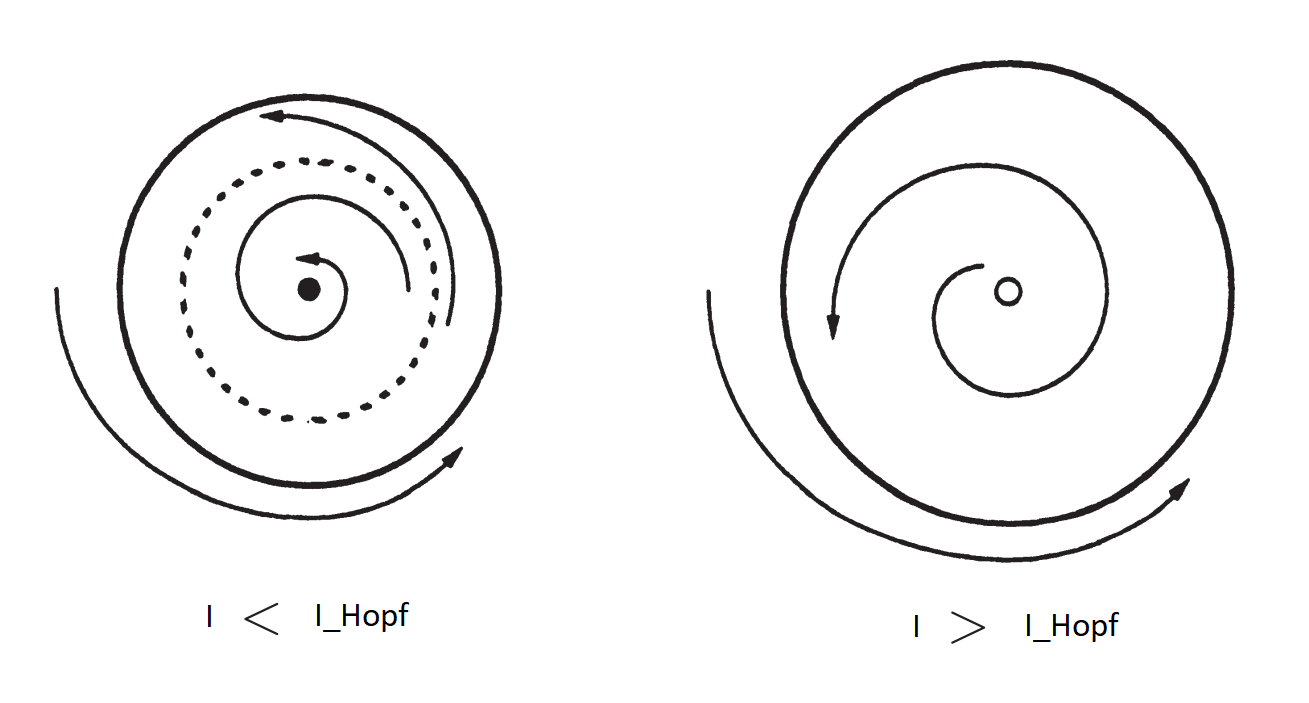
\includegraphics[width=0.5\linewidth]{Subcritical_Hopf_Bifurcation}
			\caption{Sub-critical Hopf bifurcation Visualization 	[4], for $I < I_{SH}$ there are two unstable and stable limit cycles and one stable fixed point. In $I=I_{SH}$, stable fixed point merges with unstable limit cycle and forms a new unstable fixed point for $I>I_{SH}$}
			\label{fig:subcriticalhopfbifurcation}
		\end{figure}
		
		With appropriate initial condition we can reach temporary oscillation solutions around unstable orbit near hopf bifurcations point ($I_{HP}$). The existence of this unstable cycle is shown in figures 6 and 7.
		
				
		% TODO: \usepackage{graphicx} required
		\begin{figure}[H]
			\centering
			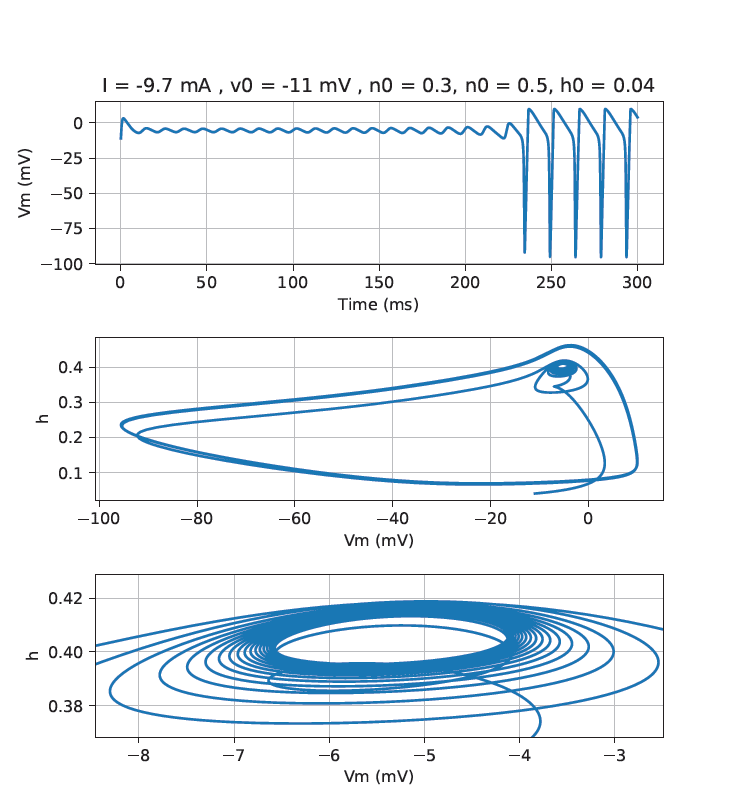
\includegraphics[width=0.5\linewidth]{SH_example}
			\caption{Simulation for I = 9.7 with a suitable chosen initial condition. System orbits near an unstable cycle around 200 time length and after that switches to the larger orbit which is stable. }
			\label{fig:shexample}
		\end{figure}
		% TODO: \usepackage{graphicx} required
		\begin{figure}[H]
			\centering
			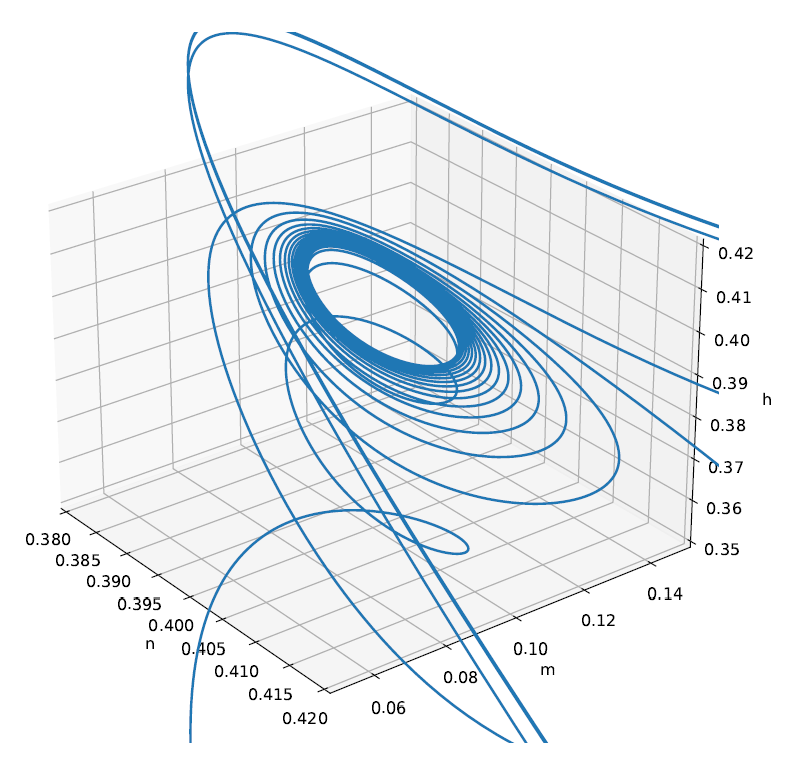
\includegraphics[width=0.5\linewidth]{SH_example_2}
			\caption{The small unstable periodic orbit around fixed point in the (m,n,h) space with the same initial point as Figure 6 and near hopf bifurcation point (I = 9.7)}
			\label{fig:shexample2}
		\end{figure}
	
	
		
		
	\section{Period Doubling Bifurcation}
		One of the ways to see period doubling bifurcation is looking at local extrema points of v(t) [6]. By simulating and recording maxima for different currnets (I) we reach figures in below: \\
		
		
		\begin{figure}[H]
			\centering
			\begin{subfigure}{0.7\textwidth}
				\centering
				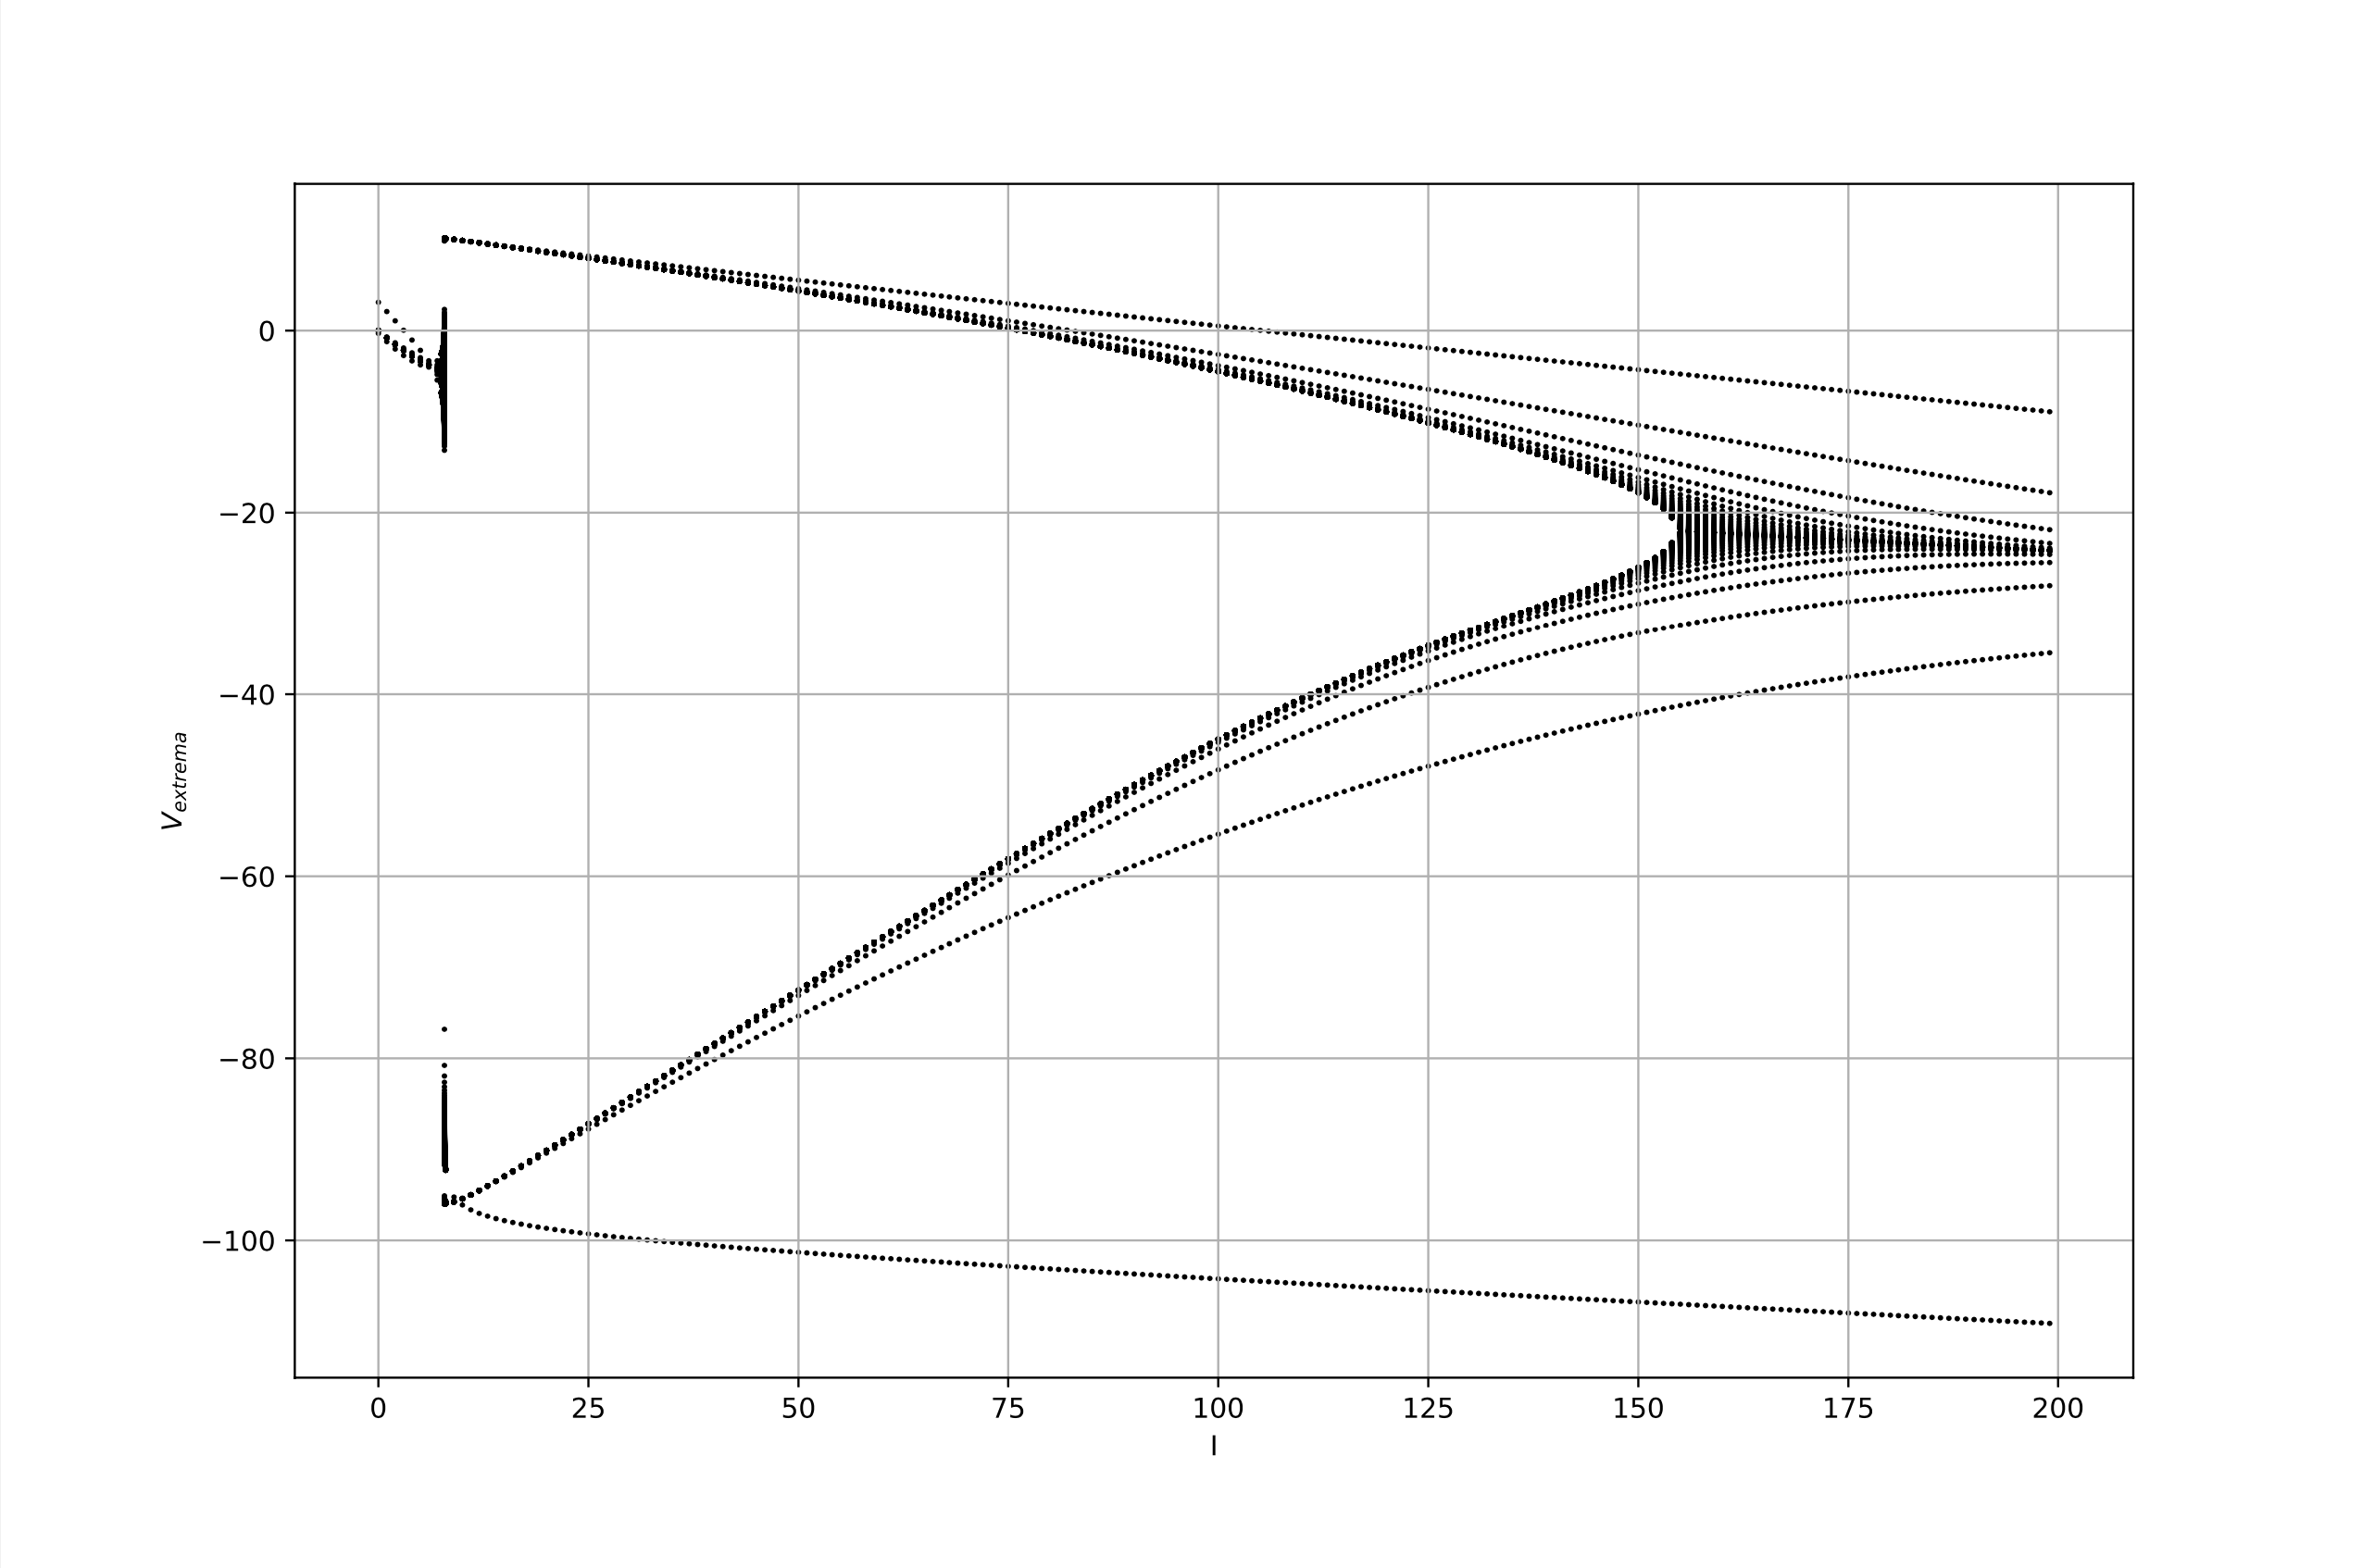
\includegraphics[width=\textwidth]{Period_doubling}
				\caption{I between 0 to 200}  
				\label{fig:mean and std of net14}
			\end{subfigure}
			\hfill
			\begin{subfigure}{0.7\textwidth}  
				\centering 
				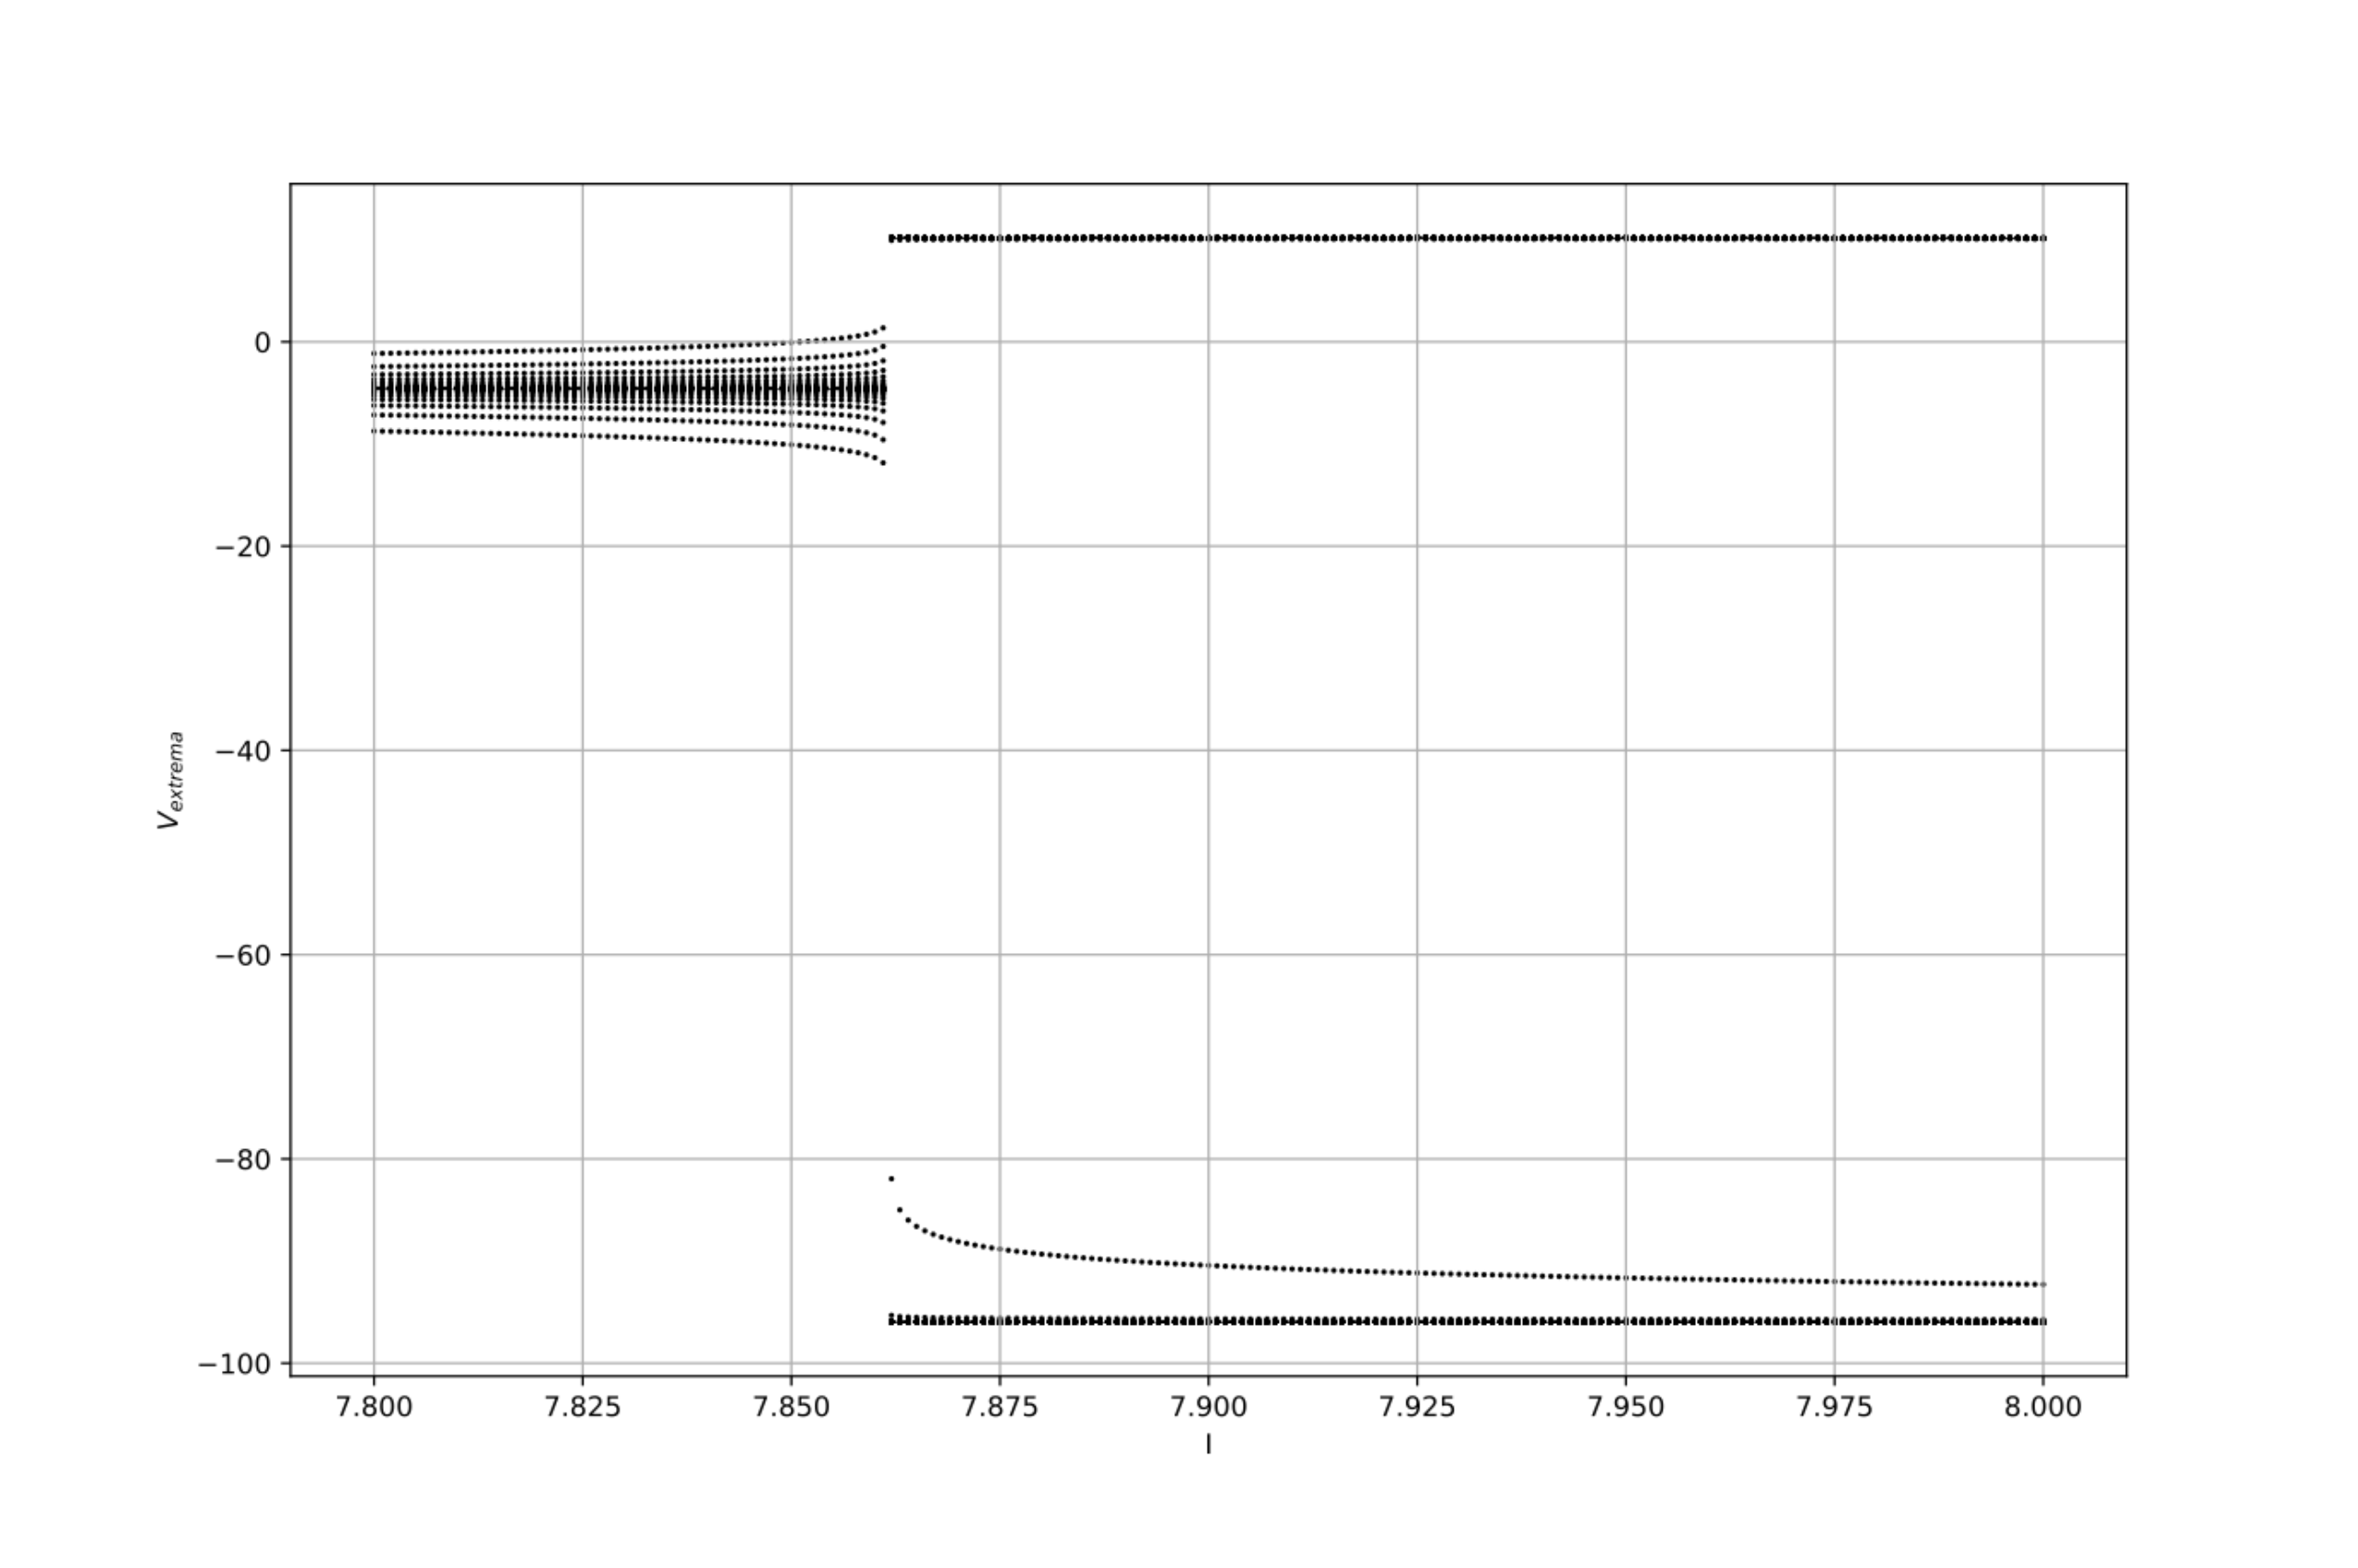
\includegraphics[width=\textwidth]{Period_doubling1}
				\caption{I between 7.8 to 8.0}   
				\label{fig:mean and std of net24}
			\end{subfigure}
			\caption{Maximum and minimum of v(t) for different I.} 
			\label{fig:mean and std nets}
		\end{figure}
		
		From Figure 8.(b), critical current is found $I_{PD} \approx 7.86$
		
	\section{Lyapunov Exponent}
		One of the necessary conditions of chaos is exponential behavior of distance between close starting points respect to time $\rightarrow |\vec{\delta}(t)| \approx \vec{\delta}_0 e^{\lambda t}$. Where the exponent factor $\lambda$ is Lyapanov exponent of the system. An N dimensional system has N different Lyapanov exponent. In this part I have explored three of them. \\
		
		\begin{figure}[H]
			\centering
			\begin{subfigure}{0.7\textwidth}
				\centering
				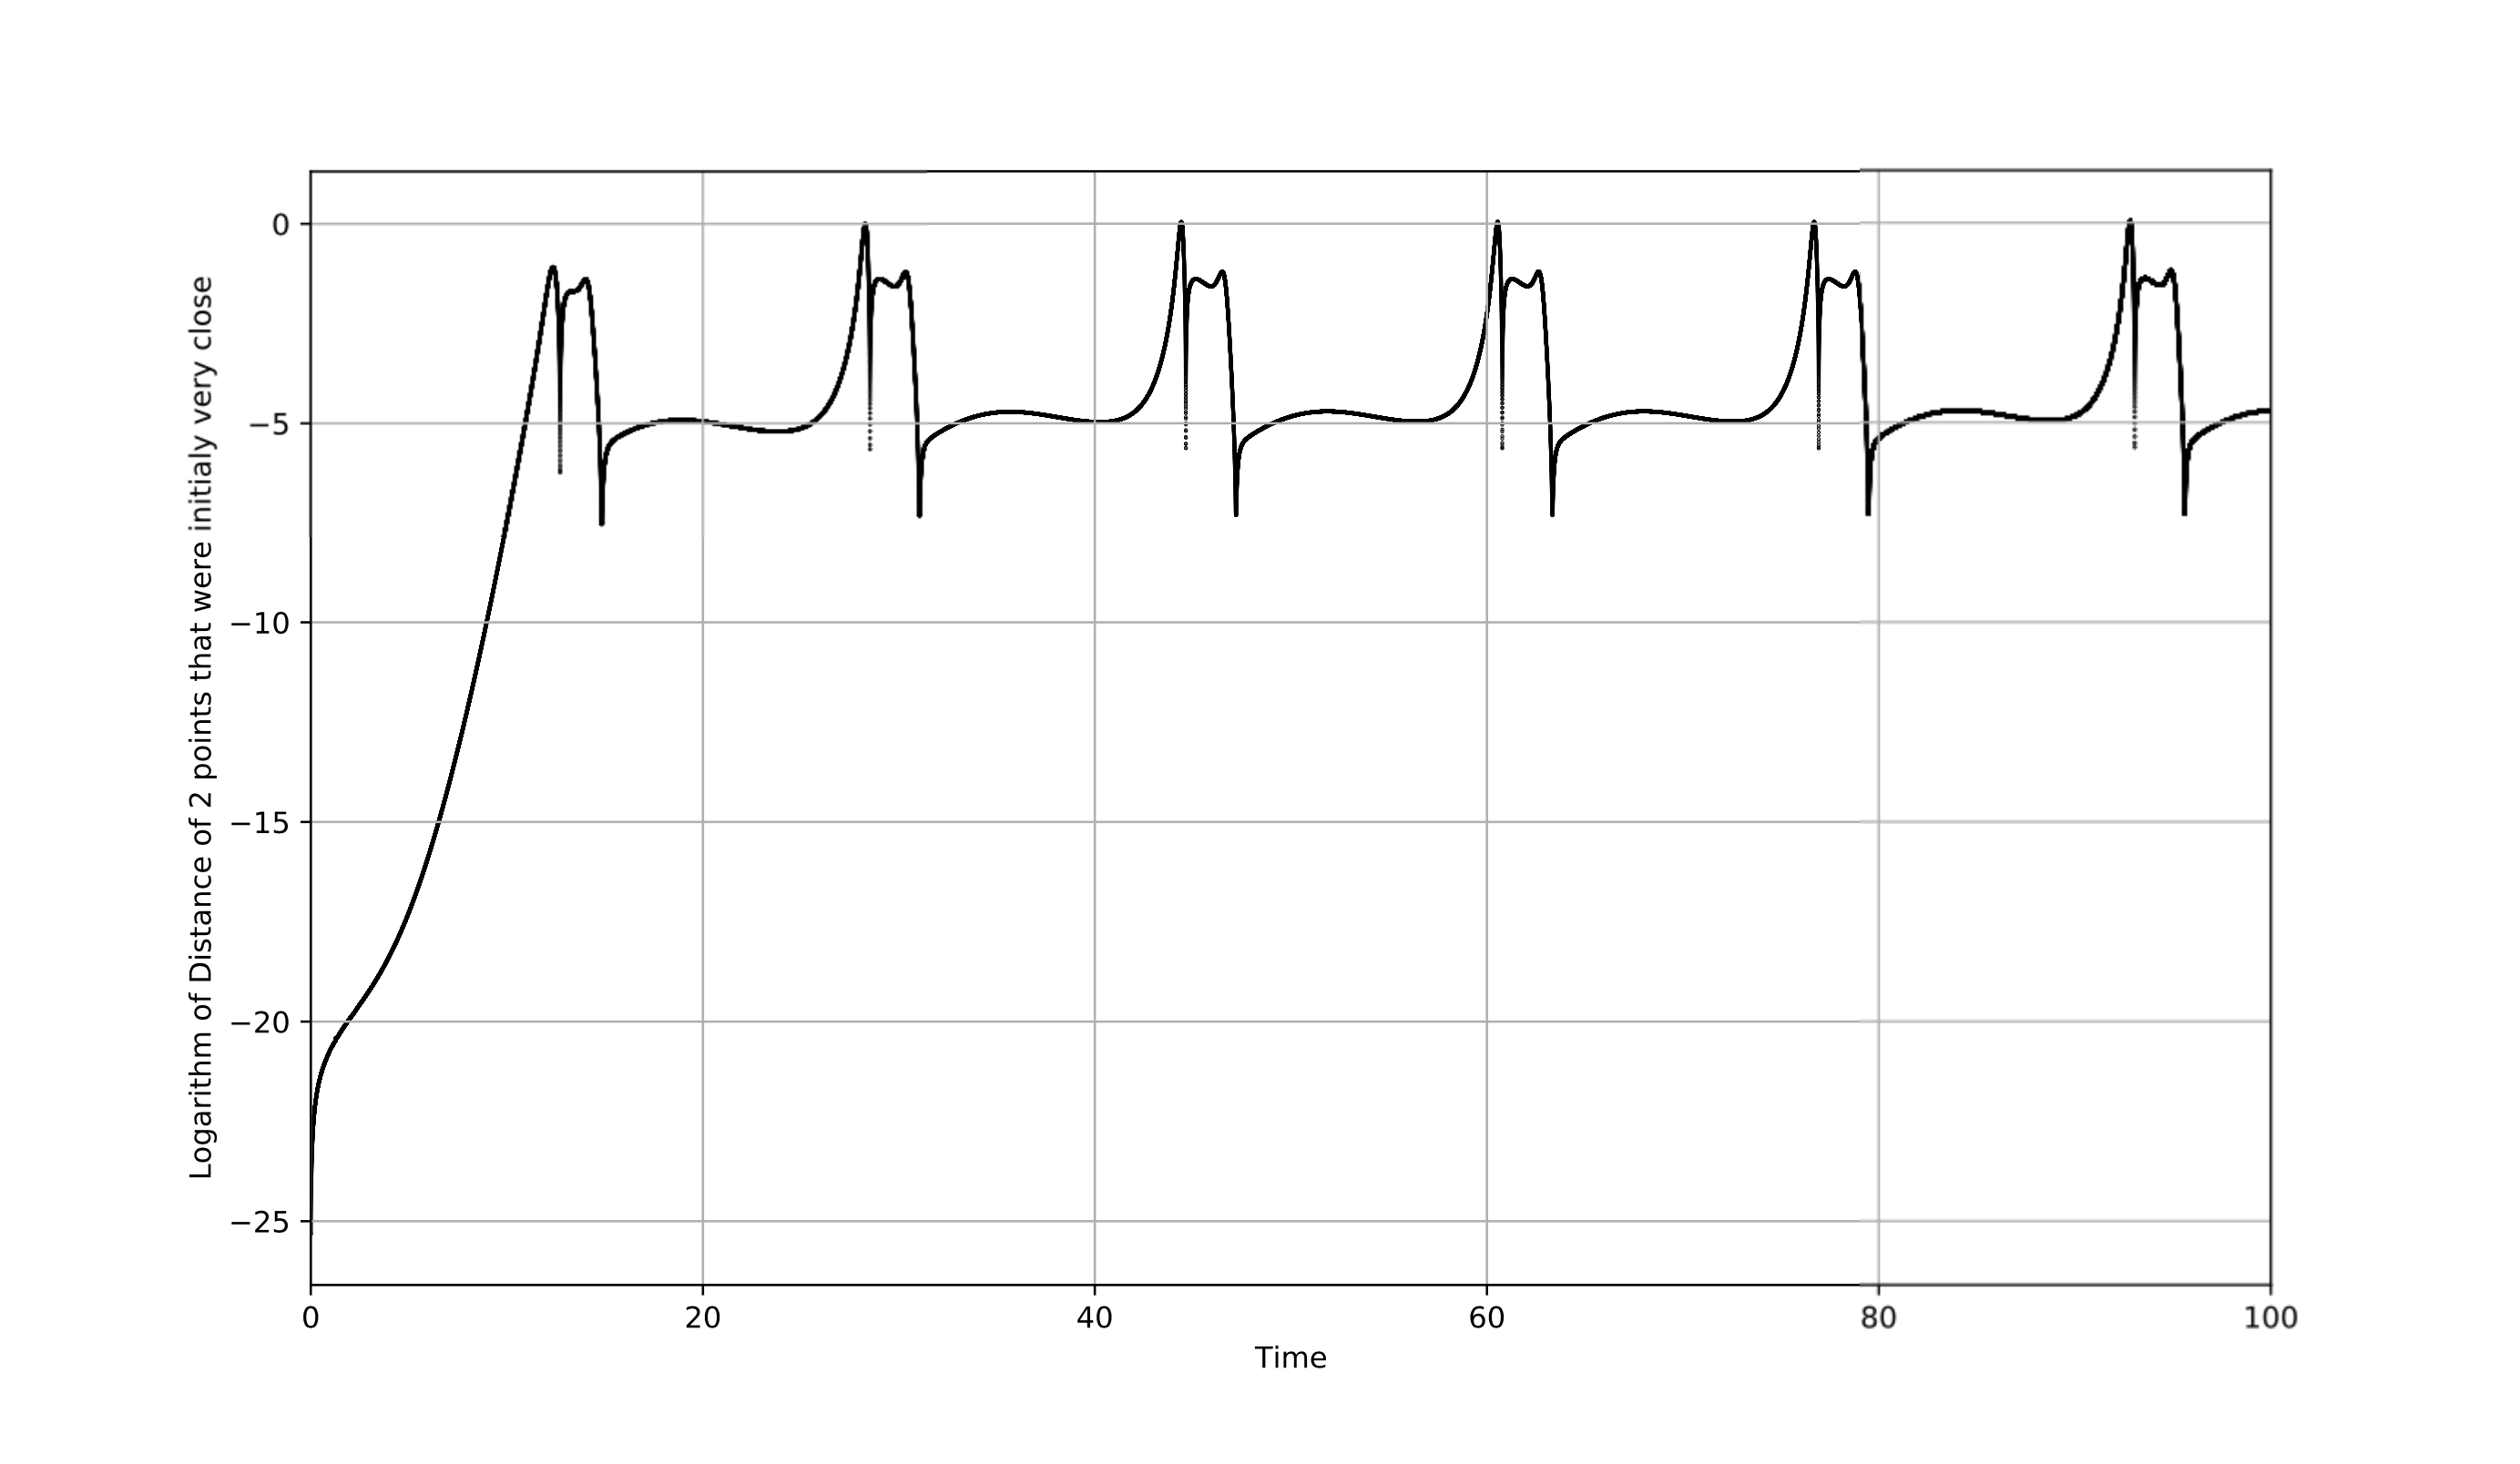
\includegraphics[width=\textwidth]{Lyapanov1}
				\caption{Initial points : [-4.5, 0.08499590453730, 0.37636277095981, 0.43229451177367] and [-4.5, 0.08499590453730, 0.37636277095981, 0.43229451177364]}  
				\label{fig:mean and std of net14}
			\end{subfigure}
			\hfill
			\begin{subfigure}{0.7\textwidth}  
				\centering 
				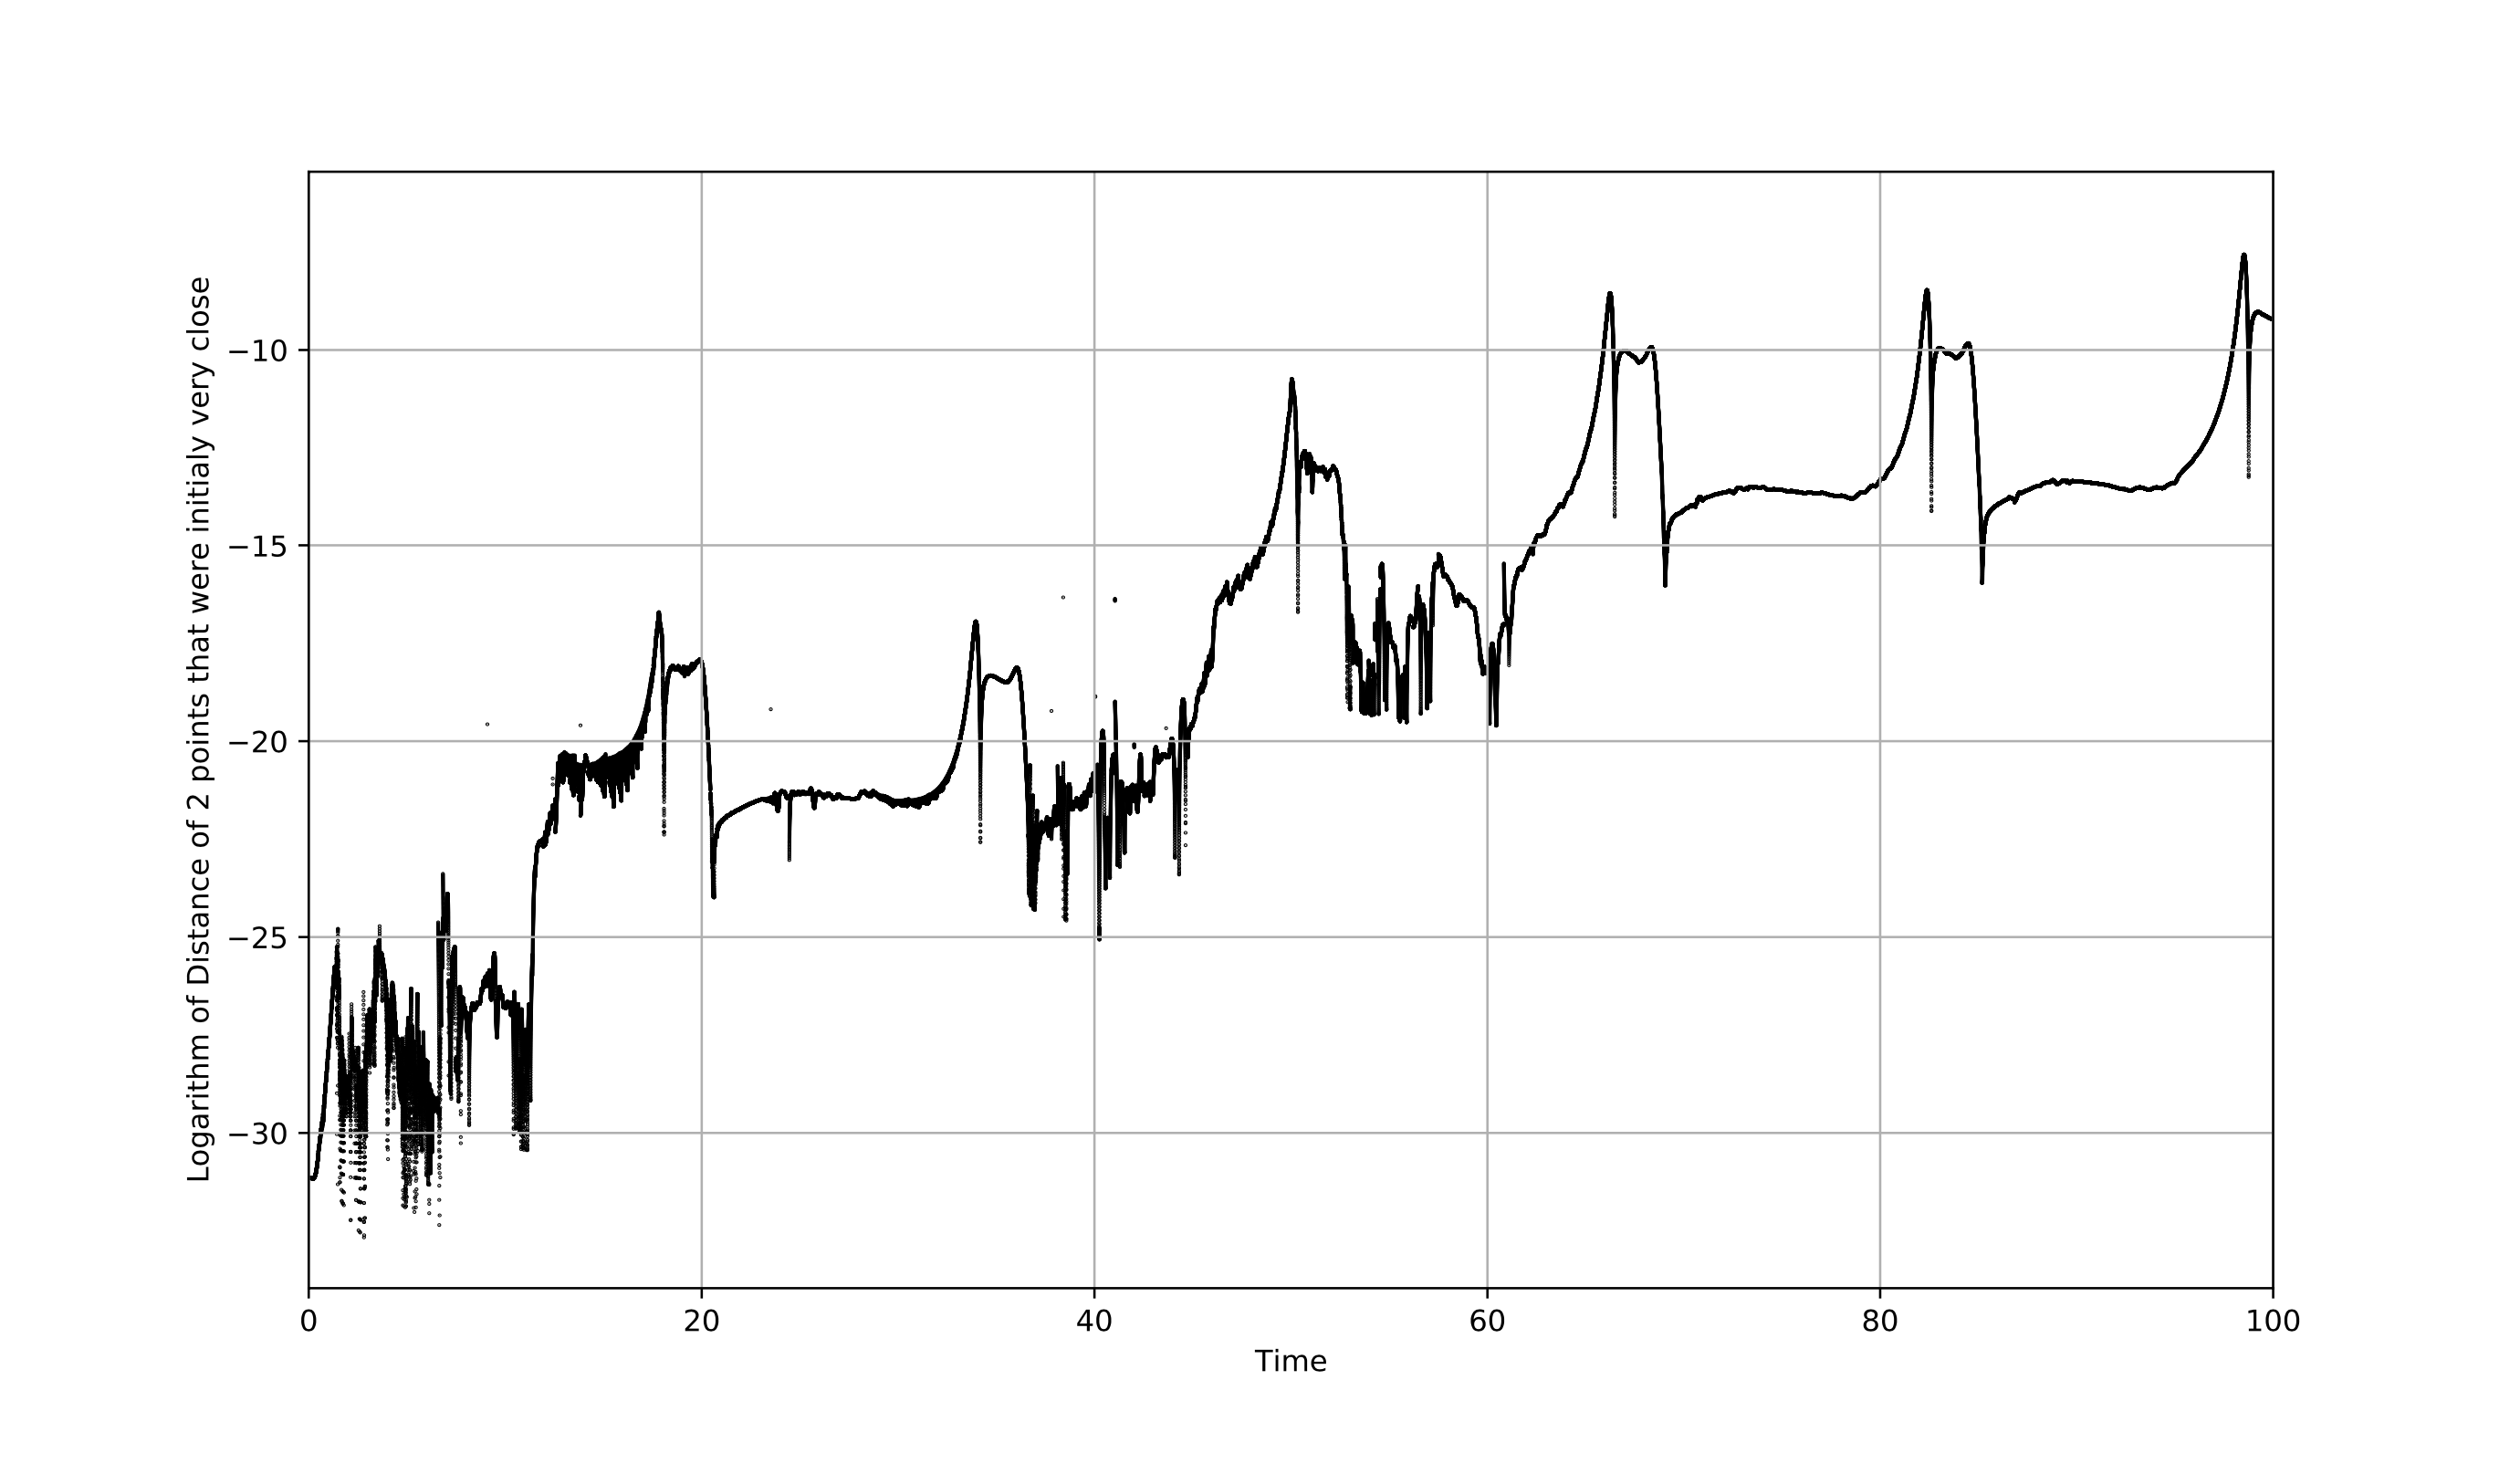
\includegraphics[width=\textwidth]{Lyapanov2}
				\caption{Initial points : [-4.5, 0, 0, 0.43229451177367] and [-4.5, 0, 0, 0.43229451177364]}   
				\label{fig:mean and std of net24}
			\end{subfigure}
			\hfill
			\begin{subfigure}{0.7\textwidth}  
				\centering 
				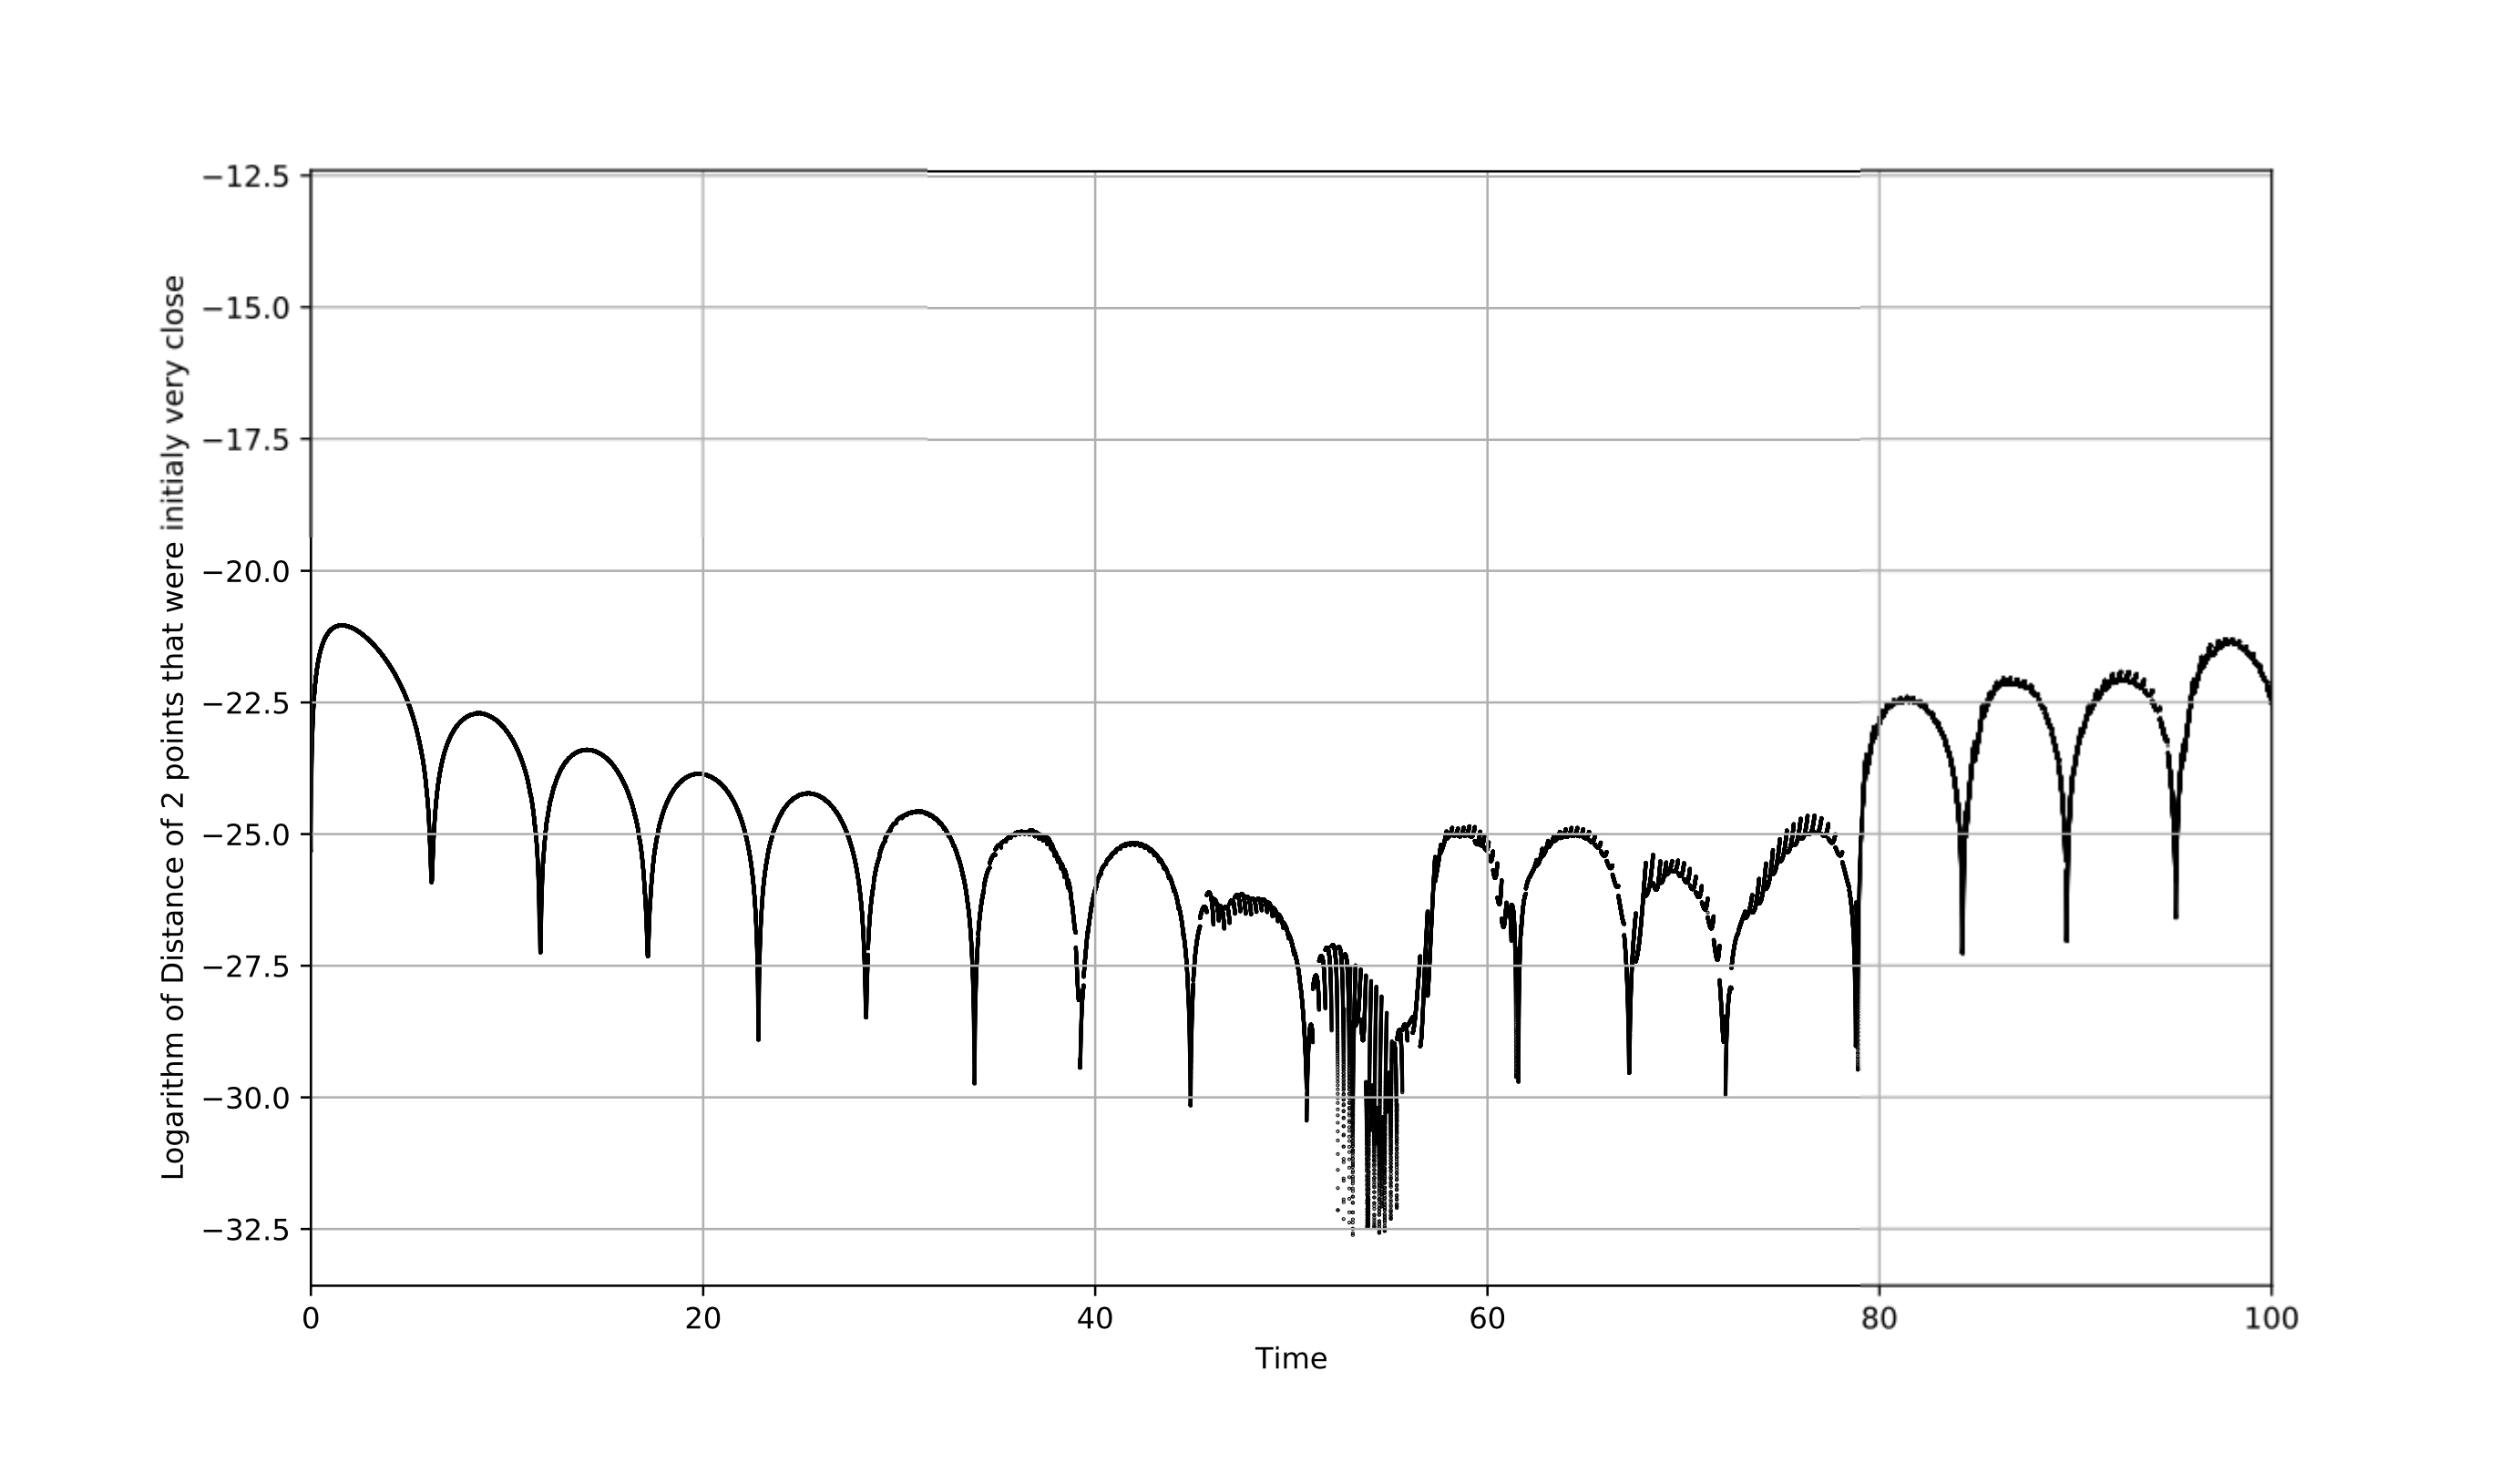
\includegraphics[width=\textwidth]{Lyapanov3}
				\caption{Initial points : [-4.5, 0.08499590453730, 0.37636277095981, 0.0.03229451177367] and [-4.5, 0.08499590453730, 0.37636277095981, 0.0.03229451177364]}   
				\label{fig:mean and std of net24}
			\end{subfigure}
			\caption{Logarithm of distance between two very close trajectories moving in 4D space versus time at current (I=7.9). (a) In this case system goes to largest orbit and the distance of two points reaches maximum value, by fitting line to the first part $\lambda \approx 1.37$ (b) $\lambda \approx0.161$ (c) In this case, two solutions converge to fixed point, $\lambda \approx 0$} 
			\label{fig:mean and std nets}
		\end{figure}

		
		
	\section{Smale Horseshoe}
		Using the more precise concept of invariant cone fields, Moser proved that a map f (Poincare discrete map) satisfying
		2 properties has a “Smale horseshoe” a hyperbolic invariant set on which f is topologically
		equivalent to the shift on two symbols[1]. I tried to use coordinates near the paper[1] coordinates and applying discrete Poincare map (computationally) defined at cross-section (v=-4.5) to find the Smale's horseshoe : 
		
				
		% TODO: \usepackage{graphicx} required
		\begin{figure}[H]
			\centering
			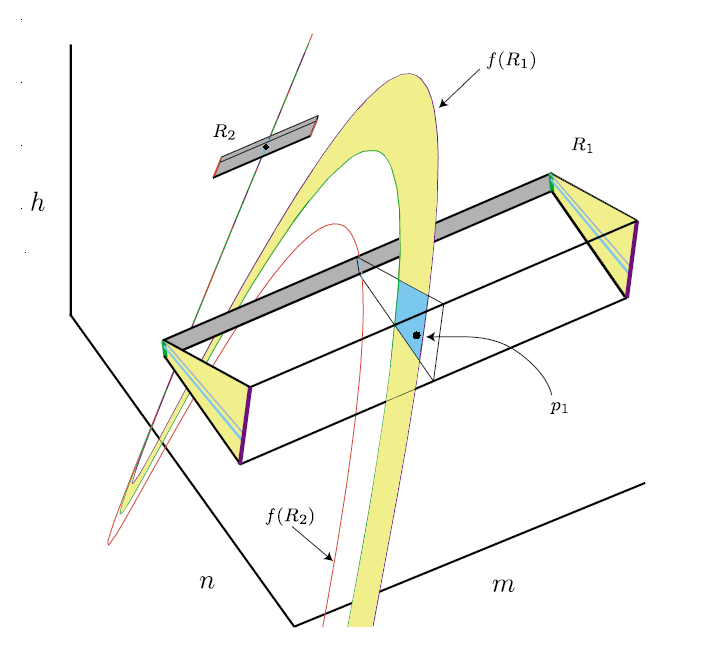
\includegraphics[width=0.6\linewidth]{smale_horseshoe}
			\caption{Paper[1] schematic view of Smale's Horseshoe in (n,m,h) discrete space}
			\label{fig:smalehorseshoe}
		\end{figure}
		
			
		
		% TODO: \usepackage{graphicx} required
		\begin{figure}[H]
			\centering
			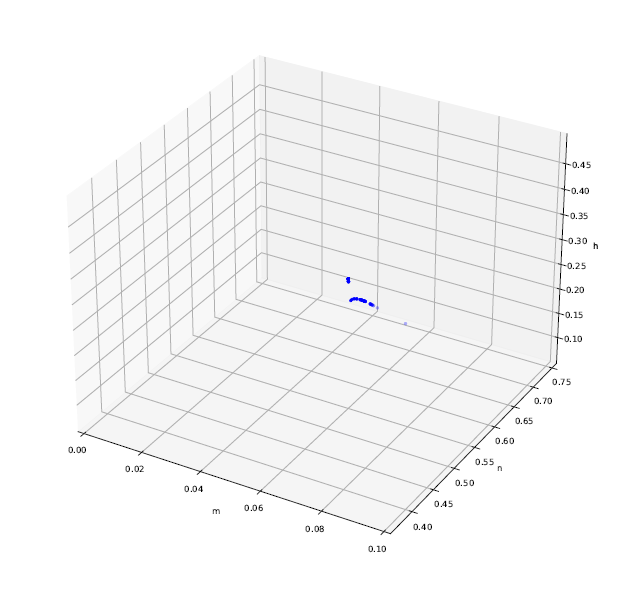
\includegraphics[width=0.7\linewidth]{smale_horseshoe2}
			\caption{The best result I could get for Smale horseshoe}
			\label{fig:smalehorseshoe2}
		\end{figure}
	
		% TODO: \usepackage{graphicx} required
		\begin{figure}[H]
			\centering
			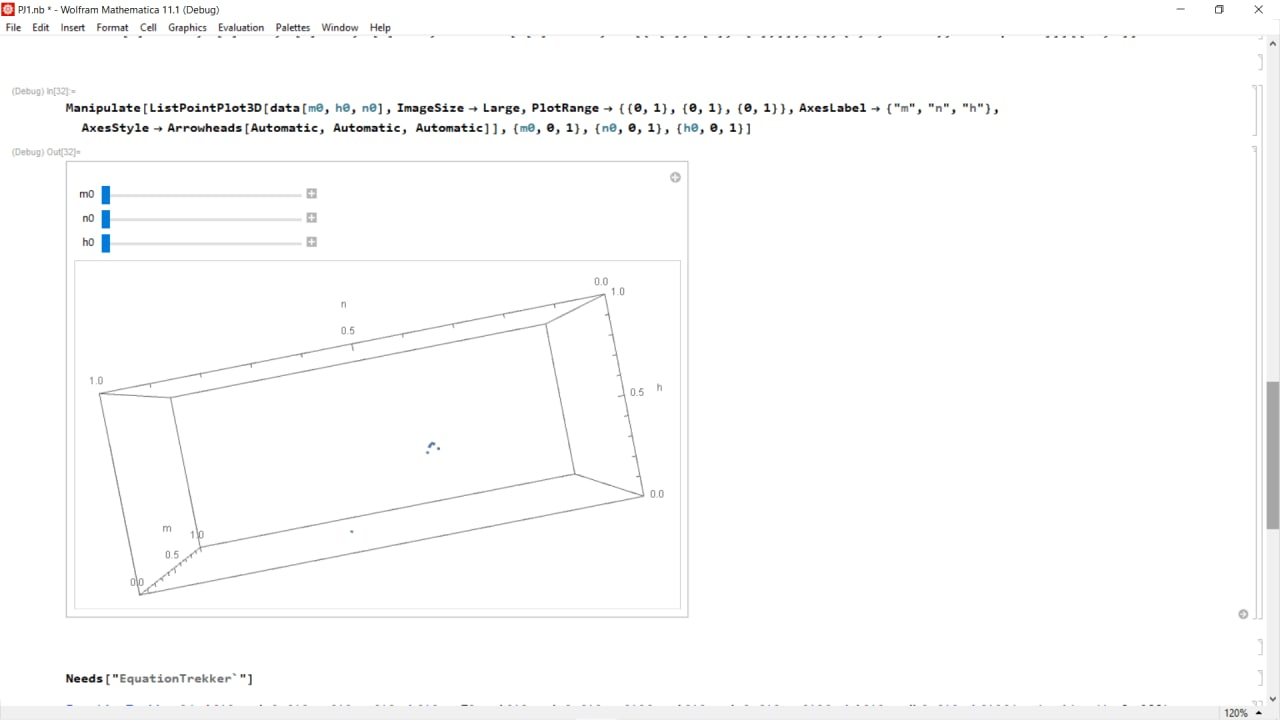
\includegraphics[width=0.7\linewidth]{photo_2022-02-04_09-05-08}
			\caption{The best result I could get for smale horseshoe}
			\label{fig:photo2022-02-0409-05-08}
		\end{figure}
	
	
	
	
	\section{Discussion}
		I could not definitely confirm that Smale horseshoe exists or not. But I found a map which is similar (figure 11 and 12). It is more likely that there is a Poincare map in HH model which has chaotic properties. The fact is chaos in HH model exists only for just a small width of current and do not forget that all this considerations are for constant current! We can modify our study to the sinusoidal input where the control parameters space becomes 2 dimensional (amplitude ($I_0$), frequency ($\omega$)).\\
		In conclusion, assume HH model is the true model for describing a single neuron and it has a chaotic region, still tuning parameters of a single neuron into that specific region is not feasible, also we could tune, we can not ignore the noise so chaotic solutions are super unstable.\\ In my opinion brain chaos is an emergent property of the population and not the single neurons so we have to look for chaos in a network of Hodgkin Huxley neurons. 
	
	\section{Methods and Challenges}
		The methods I used to derive figures and diagrams are codes in python and Matlab programming languages primarily based on Euler integration algorithm.\\
		
		\textbf{Challenges}\\
		\textbf{1.} Finding unstable orbits in this system was technically hard for me because trajectories diverge from this solutions. I searched in the Internet and find a few papers with different methods but I could not use them at the end. 
		\\
		The most popular algorithm of finding UPO (unstable periodic orbits) is the Newton-Raphson method
		with a Poincare section, which reduces a continuous dynamical system to a discrete system. Another method is to detect a UPO by stabilizing the periodic orbit in the sense of chaos control (Pyragas, 1992). Kazantsev (1998) develops a method which requires similar techniques to data assimilation, and there is also a variational method (Lan and Cvitanovic, 2004) [5].\\
		\textbf{My own raw idea to find the unstable orbits:} \\
		As we know, a dynamical system's equations of motion are time reversal n theory. So, I thought that by reversing the time arrow in computational simulation we can reverse the trajectories and reach to the unstable orbit. But simulations did not go back in time properly and they have just started to diverge after a time period (see figure )	
		  
		
		% TODO: \usepackage{graphicx} required
		\begin{figure}[H]
			\centering
			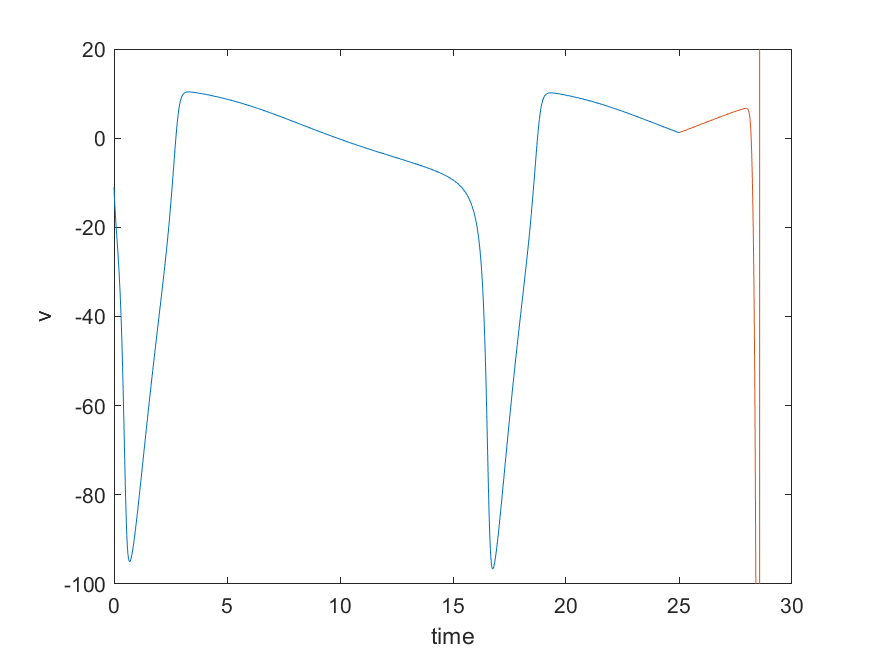
\includegraphics[width=0.7\linewidth]{reversal}
			\caption{Membrane potential versus time. At t = 25 we reverse the Euler integrator ($dt \rightarrow -dt$). We expect to see th flipped trajectory respect to t=25 axis, but after a short time simulation diverges and goes to infinity.}
			\label{fig:reversal}
		\end{figure}
		
		After previous observation I found that the integrating algorithm itself should be time reversal too! And normal Euler integrator is not time reversal. My plan for further studies is to find a time reversal algorithm in order to find UPO s.\\
		
		\textbf{2.} In the Figure below, Stable orbit in the (h, v) plane is shown. the left diagram is from paper [1] and the right one is my simulation. The problem I noticed is that, the shapes are not completely the same and I checked everything but could not find the solution. 
		
		\begin{figure}[H]
			\centering
			\begin{subfigure}{0.45\textwidth}
				\centering
				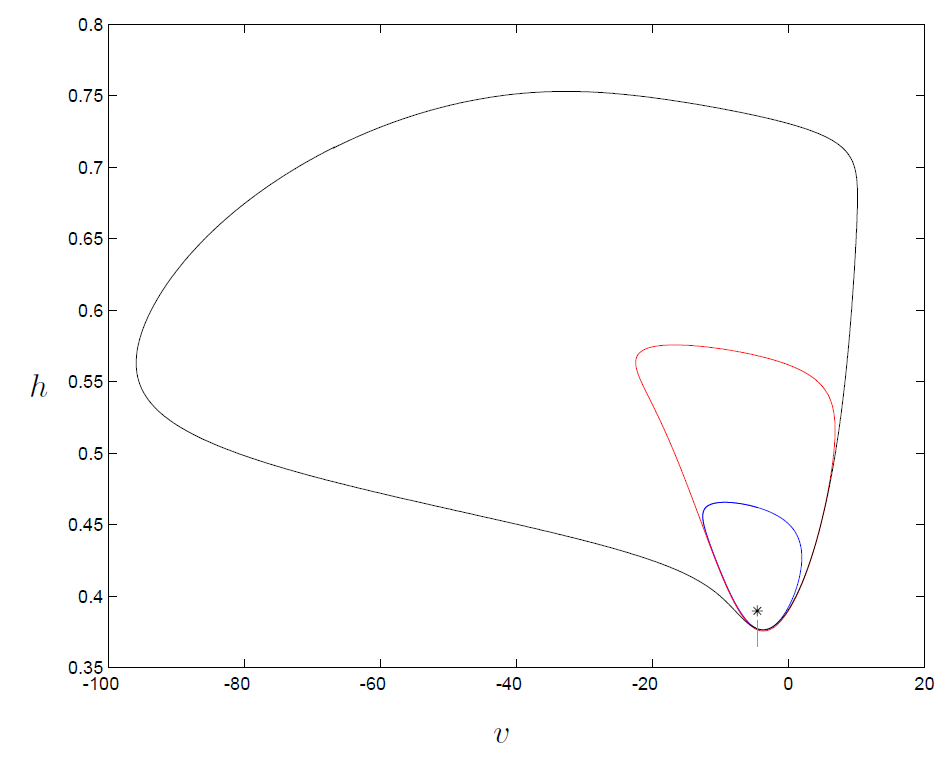
\includegraphics[width=\textwidth]{h_v}
				\caption{The paper orbits (The black one is the stable one)}  
				\label{fig:mean and std of net14}
			\end{subfigure}
			\hfill
			\begin{subfigure}{0.5\textwidth}  
				\centering 
				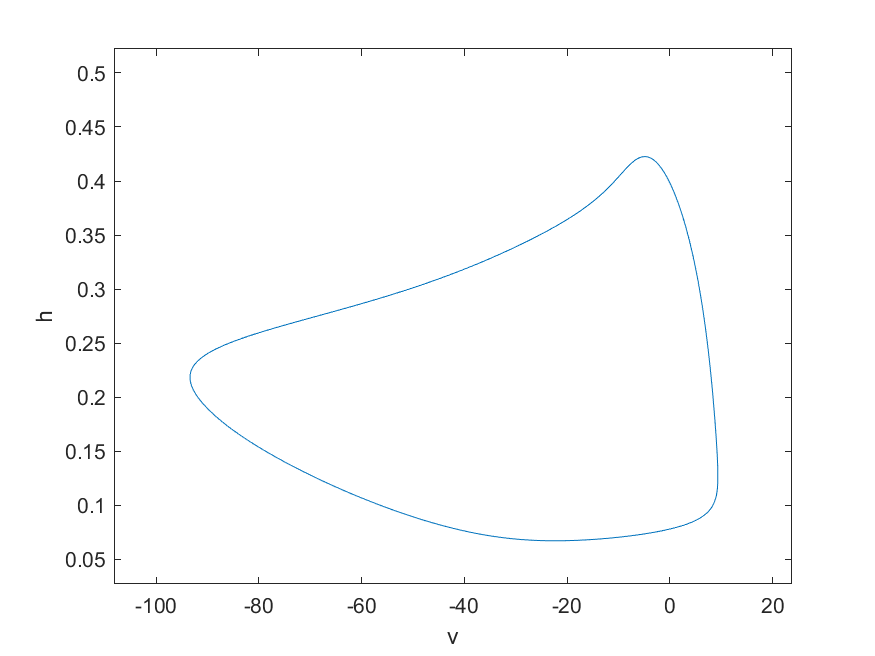
\includegraphics[width=\textwidth]{h_v_2}
				\caption{My stable orbit}   
				\label{fig:mean and std of net24}
			\end{subfigure}
			\caption{Comparison of my simulation and paper[1] result} 
			\label{fig:mean and std nets}
		\end{figure}
		
		\textbf{3.} The other challenge I encountered was the accuracy and meaningful digits in paper [1] is very high while mine is not. And the paper has not mentioned clearly how they reached those diagrams and data. So I could not reproduce the whole paper's result. 
	\section{References}
		[1] John Guckenheimer and Ricardo A. Oliva, Chaos in the Hodgkin–Huxley Model
		\\
		$[2]$ J. Guckenheimer and P. Holmes, Nonlinear Oscillations, Dynamical Systems, and Bifurcations of
		Vector Fields, Springer-Verlag, New York, 1983. 
		\\
		$[3]$ Brian Hassard, Bifurcation of Periodic Solutions of the Hodgkin-Huxley Model for the Squid Giant Axon, 1977 
		\\
		$[4]$ Steven H. Strogatz, Nonlinear Dynamics and Chaos, second edition, bifurcation revisited (p 244-287)
		\\
		$[5]$ Y. Saiki, Numerical detection of unstable periodic orbits in continuous-time
		dynamical systems with chaotic behaviors
		\\
		$[6]$
		S. Doi, S. Nabetani, S. Kumagai. , Complex nonlinear dynamics of the Hodgkin-Huxley
		equations induced by time scale changes, Biol. Cybern., 85 (2001), pp. 51-64.
	
\end{document}